% !TeX program = xelatex
% Compile with XeLaTeX (fontspec + Korean text).
% Shared Beamer style and diagrams. Compile language files with XeLaTeX.
\documentclass[aspectratio=169,10pt]{beamer}
\usepackage[no-math]{fontspec}
\setsansfont{Malgun Gothic}
\setmainfont{Malgun Gothic}
\setmonofont{Consolas}
\XeTeXlinebreaklocale "ko"
\XeTeXlinebreakskip=0pt plus 0.5pt
\usepackage{amsmath,graphicx,booktabs,tikz}
\usefonttheme{professionalfonts}
\usefonttheme[onlymath]{serif}
\usetikzlibrary{arrows.meta,positioning,calc,shapes.geometric}
\definecolor{ink}{HTML}{142938}
\definecolor{accent}{HTML}{155F85}
\definecolor{pale}{HTML}{E7F0F7}
\definecolor{collision}{HTML}{A03336}
\setbeamercolor{normal text}{fg=ink,bg=white}
\setbeamercolor{frametitle}{fg=ink}
\setbeamercolor{structure}{fg=accent}
\setbeamerfont{frametitle}{size=\Large,series=\bfseries}
\setbeamertemplate{navigation symbols}{}
\setbeamertemplate{footline}{\hfill{\color{accent}\scriptsize RMFS Architecture\quad \insertframenumber\ /\ \inserttotalframenumber}\hspace{5mm}\vspace{3mm}}
\setbeamersize{text margin left=7mm,text margin right=7mm}
\hypersetup{pdftitle={RMFS Architecture}}
\tikzset{
 phase/.style={ellipse,draw=accent,fill=pale,minimum width=23mm,minimum height=10mm,align=center,font=\small},
 terminal/.style={phase,draw=collision,fill=red!5},
 flow/.style={-{Stealth[length=2mm]},draw=accent,thick},
 ext/.style={flow,dashed},
 crash/.style={ext,draw=collision},
 lab/.style={font=\scriptsize,align=center,fill=white,inner sep=1.5pt},
 module/.style={draw=accent,fill=pale,rounded corners=2pt,minimum width=34mm,minimum height=13mm,align=center}
}
\newcommand{\MRobotDiagram}{%
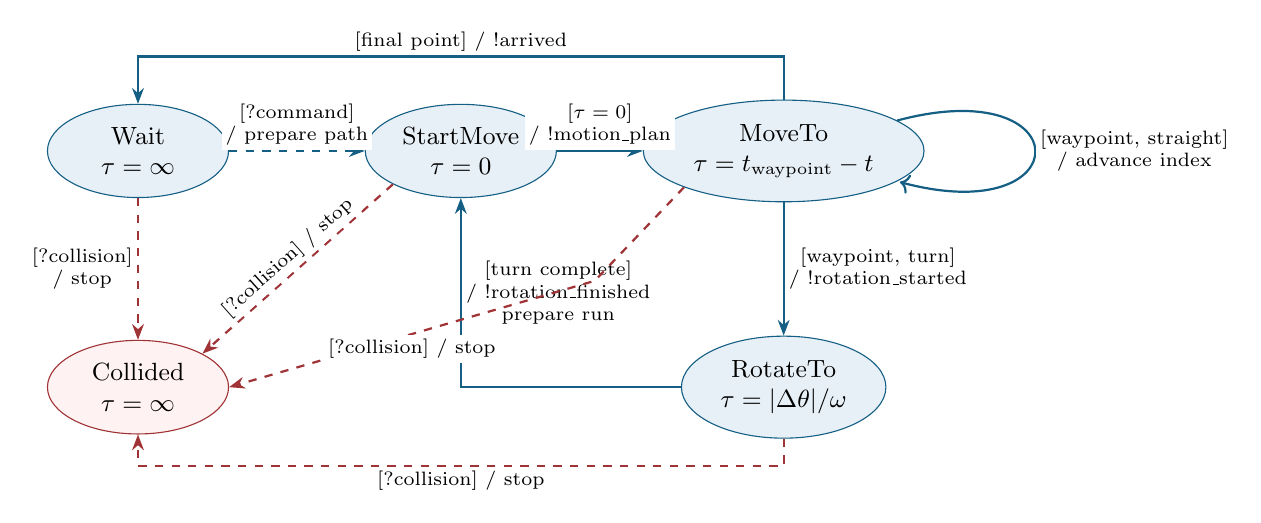
\begin{tikzpicture}[x=1cm,y=1cm]
\node[phase] (w) at (0,3) {Wait\\$\tau=\infty$};
\node[phase] (s) at (4.1,3) {StartMove\\$\tau=0$};
\node[phase] (m) at (8.2,3) {MoveTo\\$\tau=t_{\rm waypoint}-t$};
\node[phase] (r) at (8.2,0) {RotateTo\\$\tau=|\Delta\theta|/\omega$};
\node[terminal] (c) at (0,0) {Collided\\$\tau=\infty$};
\draw[ext] (w)--node[lab,above]{[?command]\\ / prepare path}(s);
\draw[flow] (s)--node[lab,above]{[$\tau=0$]\\ / !motion\_plan}(m);
\draw[flow] (m) edge[loop right] node[lab,right]{[waypoint, straight]\\ / advance index}(m);
\draw[flow] (m)--node[lab,right]{[waypoint, turn]\\ / !rotation\_started}(r);
\draw[flow] (r.west)--(4.1,0) -- node[lab,right]{[turn complete]\\ / !rotation\_finished\\prepare run}(s.south);
\draw[flow] (m.north)--(8.2,4.2)--node[lab,above]{[final point] / !arrived}(0,4.2)--(w.north);
\draw[crash] (w.south)--node[lab,left]{[?collision]\\ / stop}(c.north);
\draw[crash] (s.south west)--node[lab,above,sloped]{[?collision] / stop}(c.north east);
\draw[crash] (m.south west)--(5.8,1.35)--node[lab,below]{[?collision] / stop}(c.east);
\draw[crash] (r.south)--(8.2,-1)--node[lab,below]{[?collision] / stop}(0,-1)--(c.south);
\end{tikzpicture}}
\newcommand{\PSensorDiagram}{%
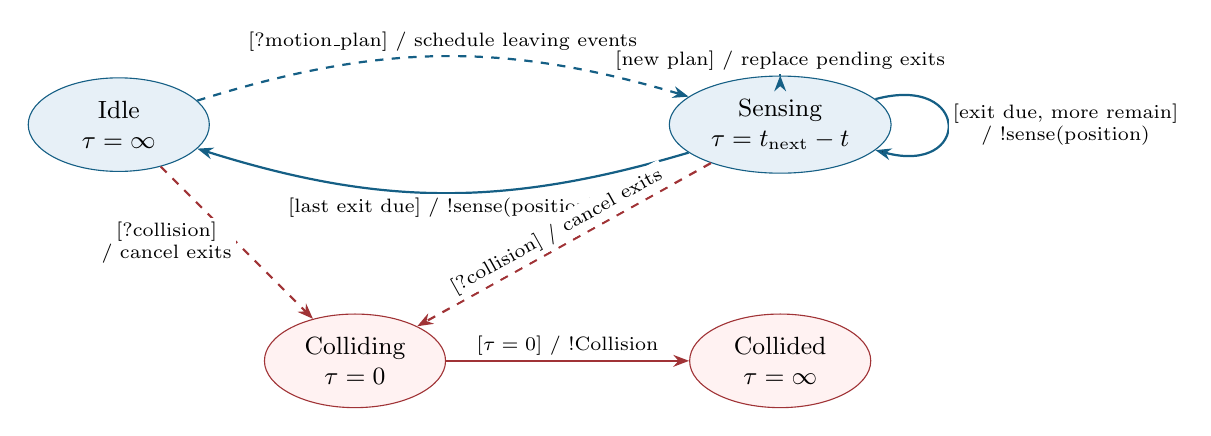
\begin{tikzpicture}[x=1cm,y=1cm]
\node[phase] (i) at (0,3) {Idle\\$\tau=\infty$};
\node[phase] (s) at (8.4,3) {Sensing\\$\tau=t_{\rm next}-t$};
\node[terminal] (g) at (3,0) {Colliding\\$\tau=0$};
\node[terminal] (c) at (8.4,0) {Collided\\$\tau=\infty$};
\draw[ext] (i) to[bend left=17] node[lab,above]{[?motion\_plan] / schedule leaving events}(s);
\draw[flow] (s) to[bend left=17] node[lab,below]{[last exit due] / !sense(position)}(i);
\draw[flow] (s) edge[loop right,looseness=5] node[lab,right]{[exit due, more remain]\\ / !sense(position)}(s);
\draw[ext] (s.north) to[out=120,in=60,looseness=3] node[lab,above]{[new plan] / replace pending exits}(s.north);
\draw[crash] (i)--node[lab,left]{[?collision]\\ / cancel exits}(g);
\draw[crash] (s)--node[lab,sloped,above]{[?collision] / cancel exits}(g);
\draw[flow,draw=collision] (g)--node[lab,above]{[$\tau=0$] / !Collision}(c);
\end{tikzpicture}}
\newcommand{\Profiles}{%
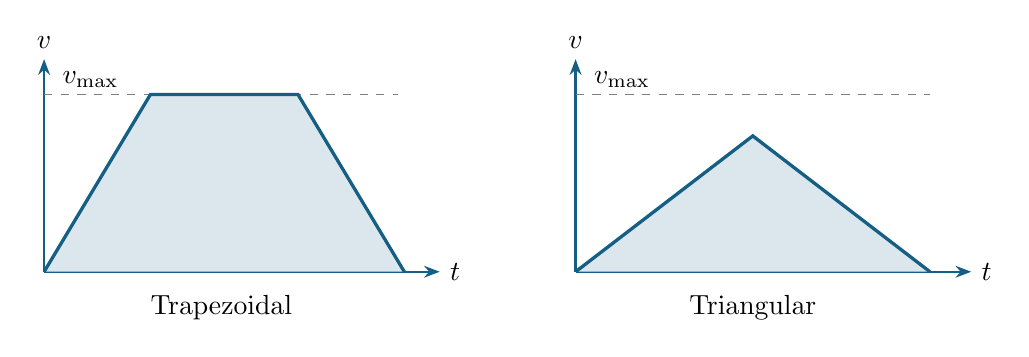
\begin{tikzpicture}[x=0.75cm,y=0.75cm]
\foreach \x in {0,9}{
 \draw[flow] (\x,0)--++(6.7,0) node[right] {$t$};
 \draw[flow] (\x,0)--++(0,3.6) node[above] {$v$};
 \draw[dashed,gray] (\x,3)--++(6,0);
}
\fill[accent!15] (0,0)--(1.8,3)--(4.3,3)--(6.1,0)--cycle;
\draw[accent,very thick] (0,0)--(1.8,3)--(4.3,3)--(6.1,0);
\fill[accent!15] (9,0)--(12,2.3)--(15,0)--cycle;
\draw[accent,very thick] (9,0)--(12,2.3)--(15,0);
\node at (3,-.6) {Trapezoidal};
\node at (12,-.6) {Triangular};
\node[anchor=west] at (.15,3.25) {$v_{\max}$};
\node[anchor=west] at (9.15,3.25) {$v_{\max}$};
\end{tikzpicture}}
\newcommand{\shot}[1]{\includegraphics[width=\linewidth,height=5.65cm,keepaspectratio]{assets/#1.png}}


\usetikzlibrary{decorations.pathreplacing}
\title{RMFS Architecture}
\date{2026-11-18}
\begin{document}

\begin{frame}[plain]
\centering
{\color{accent}\LARGE Part 1\par}\vspace{8mm}
{\LARGE Introduction to RMFS\par Modeling and Control\par}
\end{frame}


\begin{frame}{RMFS Architecture}

\begin{center}
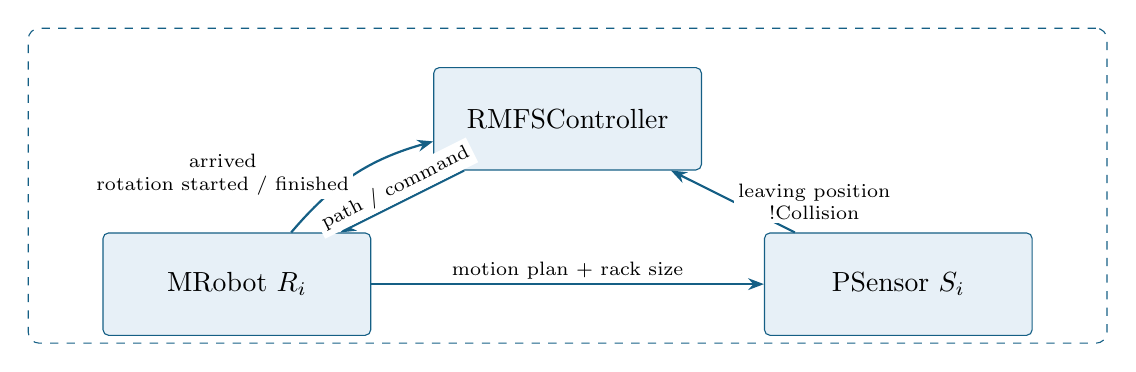
\begin{tikzpicture}
\node[module] (c) at (0,2.1) {RMFSController};
\node[module] (r) at (-4.2,0) {MRobot $R_i$};
\node[module] (s) at (4.2,0) {PSensor $S_i$};
\draw[flow] (c)--node[lab,above,sloped]{path / command}(r);
\draw[flow] (r) to[bend left=17] node[lab,left]{arrived\\rotation started / finished}(c);
\draw[flow] (r)--node[lab,above]{motion plan + rack size}(s);
\draw[flow] (s)--node[lab,right]{leaving position\\!Collision}(c);
\node[draw=accent,dashed,rounded corners,minimum width=13.7cm,minimum height=4cm] at (0,1.25) {};
\end{tikzpicture}
\end{center}

\small RMFS는 Coupled DEVS이며 제어기와 물리 이동물체별 MRobot--PSensor 한 쌍으로 구성된다.
MRobot은 운동을 실행하고 PSensor는 이탈 시점의 중심 좌표를 보고한다. MRobot의 3D 모습은 애칭으로 \textbf{Frogeye (Frogy)}라 부른다.
현재 실험은 \texttt{TestController}를 사용한다. 설계된 RMFSController 내부에는
RobotPathPlanner, TrafficManager와 공유 RoadMap이 있다.\par\smallskip Grid는 제어점 $4\times4$개, 셀 $3\times3$개이며 2 m 간격의 $6\times6$ m 크기다.
\end{frame}

\begin{frame}{MRobot의 phase 상태 천이}
\centering\resizebox{.95\linewidth}{!}{\MRobotDiagram}
\par\medskip\raggedright\small
화살표는 [guard] / action으로 표시한다. 점선은 외부 입력 전이다.
같은 방향으로 이어지는 구간에서는 속도를 유지하고, 직선 주행의 시작과 끝에서 가감속한다.
충돌하면 자세를 고정하고 운동 예약을 취소한다. 본체가 회전해도 랙 방향은 유지한다.
{\scriptsize $t$는 현재 시각, $t_{\rm waypoint}$는 다음 경유점 시각, $\Delta\theta$는 회전각, $\omega$는 회전 속도다.}
\end{frame}

\begin{frame}{PSensor의 phase 상태 천이}
\centering\resizebox{!}{4.2cm}{\PSensorDiagram}
\par\medskip\raggedright\small
이탈 이벤트만 예약한다. \texttt{!sense}는 이탈 시점의 이동물체 중심 좌표를 보낸다.
새 운동 계획을 받으면 미래 이탈 예약을 교체한다.
충돌 입력 시 예약을 취소하고 같은 시뮬레이션 시각에 \texttt{!Collision}을 보고한다.
예약된 이탈이 없으면 다음 이벤트 시각은 무한대다. $t_{\rm next}$는 다음 이탈 시각, $t$는 현재 시각이다.
\end{frame}

\begin{frame}{MRobot의 가속·등속·감속 프로파일}
\begin{center}\resizebox{.82\linewidth}{!}{\Profiles}\end{center}
\[
v_p=\min\!\left(v_{\max},\sqrt{\frac{2D}{1/a+1/b}}\right),
\qquad d_a=\frac{v_p^2}{2a},\quad d_b=\frac{v_p^2}{2b}.
\]
\[
T=\frac{v_p}{a}+\frac{D-d_a-d_b}{v_p}+\frac{v_p}{b},
\qquad T_{\rm turn}=\frac{|\Delta\theta|}{\omega}.
\]
\footnotesize
$D$는 한 번 가감속하는 연속 직선 주행의 총거리[m]다.
$a,b>0$는 가속도와 감속도 크기[m/s$^2$]다.
$v_{\max}$는 제한속도, $v_p$는 실제 도달 최고속도[m/s]다.
$d_a,d_b$는 가속·감속 거리[m], $T$는 직선 주행시간[s]이다.
$\Delta\theta$는 방향 변화각이며 $\omega$는 같은 각도 단위로 표현한 회전 속도다.
\end{frame}

\begin{frame}{PSensor의 경로상 제어점 이탈 보고}

\begin{center}
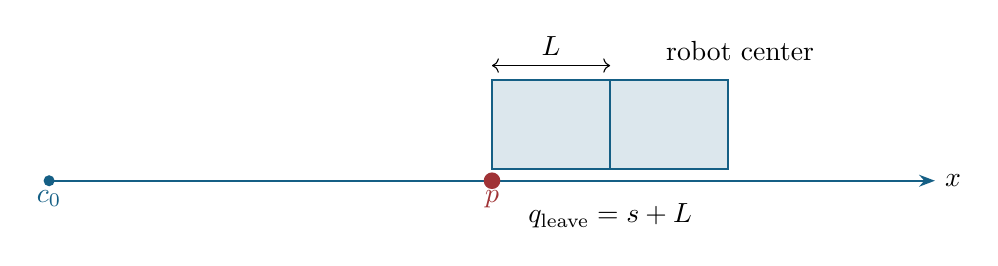
\begin{tikzpicture}[x=.75cm,y=.75cm]
\draw[flow] (0,0)--(15,0) node[right] {$x$};
\fill[accent!15] (7.5,.2) rectangle (11.5,1.7);
\draw[accent,thick] (7.5,.2) rectangle (11.5,1.7);
\draw[accent,thick] (9.5,.2)--(9.5,1.7);
\node at (11.7,2.2) {robot center};
\draw[<->] (7.5,1.95)--node[above] {$L$}(9.5,1.95);
\fill[collision] (7.5,0) circle (3pt) node[below] {$p$};
\fill[accent] (0,0) circle (2pt) node[below] {$c_0$};
\node at (9.5,-.6) {$q_{\rm leave}=s+L$};
\end{tikzpicture}
\end{center}

\[
s=(p-c_0)\cdot u,\qquad q_{\rm leave}=s+L,\qquad
t_{\rm leave}=t_0+T(q_{\rm leave}).
\]
\footnotesize
$p$는 제어점 좌표, $c_0$는 직선 주행 시작 시각 $t_0$의 이동물체 중심,
$u$는 이동 단위 방향이다. $s$는 진행 방향으로 잰 제어점까지의 부호 있는 거리다.
$q_{\rm leave}$는 이탈할 때까지 중심의 이동 거리이며 $T(q)$는 그 거리의 도달 소요시간이다.
$t_{\rm leave}$는 절대 이벤트 시각, 보고 좌표는 $c_{\rm leave}=c_0+u q_{\rm leave}$다.
\par\medskip
\textbf{현재 실험은 랙 적재 여부와 관계없이 $L=0.75$ m를 적용한다.}
생성자로 받은 1.5 m 랙 치수에서 계산한다.
$0\le q_{\rm leave}<D$이면 예약하며, 정지점 이탈은 다음 주행에서 다시 판단한다.

\end{frame}

\begin{frame}{가속·등속·감속 구간의 이탈 시각}
\[
T(q)=
\begin{cases}
\sqrt{\dfrac{2q}{a}},&0\le q\le d_a,\\[2mm]
\dfrac{v_p}{a}+\dfrac{q-d_a}{v_p},&d_a<q<D-d_b,\\[2mm]
T-\sqrt{\dfrac{2(D-q)}{b}},&D-d_b\le q\le D .
\end{cases}
\]
\footnotesize $q$는 직선 주행 시작 후 중심의 이동 거리이며 $T(q)$는 도달 소요시간이다.
$D,a,b,v_p,d_a,d_b,T$는 4장에서 정의했다. $q=s+L$을 대입하며 출발점이면 $s=0$이다.
\[
L=0.75\ {\rm m},\quad a=b=0.41\ {\rm m/s^2}
\ \Rightarrow\ T(L)=1.912730\ {\rm s}.
\]
\small 주행 시작 시 수식으로 시각을 예약하고 엔진은 해당 이벤트로 전진한다.
Viewer는 애니메이션을 위해 위치를 샘플링한다.
\end{frame}

\begin{frame}{RMFSController의 내부 구성}
\begin{center}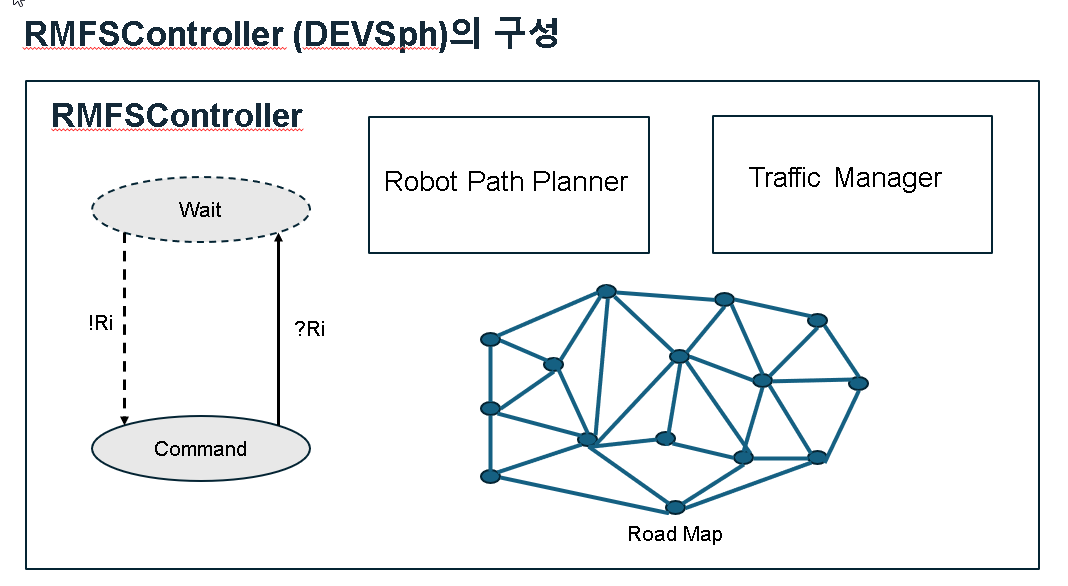
\includegraphics[width=.88\linewidth,height=5.4cm,keepaspectratio]{assets/RMFSController.png}\end{center}
\small 제공된 설계 그림이다. RobotPathPlanner와 TrafficManager가 RoadMap을 공유한다.
현재 예제는 TestController를 사용하며, 제어기 상태 천이는 추후 구체화한다.
\end{frame}

\begin{frame}{Frogy -- 중앙선 직진}
\begin{columns}[T,onlytextwidth]
\begin{column}{.70\textwidth}\shot{straight}\end{column}
\begin{column}{.28\textwidth}\small 경로 $(0,2)\to(3,2)$\par\medskip 이동 거리 6 m\par 회전 0회\par 랙 없음\par\medskip\textbf{도착시간}\par\textbf{7.651초}\par\medskip 캡처 시각 $t=3.800$초.\end{column}
\end{columns}
\vspace{1mm}
{\tiny\texttt{\detokenize{01_01_RobotPath_Straight}}\par \texttt{\detokenize{python -m examples.RMFS.Tests.01_01_RobotPath_Straight --no-rack}}\par 빈 이동물체가며 초기 방향은 첫 선분에 정렬한다. $v_{\max}=2\,\mathrm{m/s}$, $a=b=0.41\,\mathrm{m/s^2}$, $\omega=45^\circ/\mathrm{s}$.}
\end{frame}

\begin{frame}{Frogy -- 왼쪽 위에서 오른쪽 아래로 ZigZag}
\begin{columns}[T,onlytextwidth]
\begin{column}{.70\textwidth}\shot{zigzag}\end{column}
\begin{column}{.28\textwidth}\small 경로 $(0,3)\to(1,3)\to(1,2)\to\cdots\to(3,0)$\par\medskip 이동 거리 12 m\par 회전 5회\par 랙 없음\par\medskip\textbf{도착시간}\par\textbf{36.504초}\par\medskip 캡처 시각 $t=18.000$초.\end{column}
\end{columns}
\vspace{1mm}
{\tiny\texttt{\detokenize{01_02_RobotPath_LeftTop_RightBottom_ZigZag}}\par \texttt{\detokenize{python -m examples.RMFS.Tests.01_02_RobotPath_LeftTop_RightBottom_ZigZag --no-rack}}\par 빈 이동물체가며 초기 방향은 첫 선분에 정렬한다. $v_{\max}=2\,\mathrm{m/s}$, $a=b=0.41\,\mathrm{m/s^2}$, $\omega=45^\circ/\mathrm{s}$.}
\end{frame}

\begin{frame}{Frogy -- 왼쪽·아랫변 L자 경로}
\begin{columns}[T,onlytextwidth]
\begin{column}{.70\textwidth}\shot{lpath}\end{column}
\begin{column}{.28\textwidth}\small 경로 $(0,3)\to(0,0)\to(3,0)$\par\medskip 이동 거리 12 m\par 회전 1회\par 랙 없음\par\medskip\textbf{도착시간}\par\textbf{17.302초}\par\medskip 캡처 시각 $t=8.500$초.\end{column}
\end{columns}
\vspace{1mm}
{\tiny\texttt{\detokenize{01_03_RobotPath_LeftTop_RightBottom_Straight_L}}\par \texttt{\detokenize{python -m examples.RMFS.Tests.01_03_RobotPath_LeftTop_RightBottom_Straight_L --no-rack}}\par 빈 이동물체가며 초기 방향은 첫 선분에 정렬한다. $v_{\max}=2\,\mathrm{m/s}$, $a=b=0.41\,\mathrm{m/s^2}$, $\omega=45^\circ/\mathrm{s}$.}
\end{frame}

\begin{frame}{Frogy -- 두 칸 왕복과 180도 회전}
\begin{columns}[T,onlytextwidth]
\begin{column}{.70\textwidth}\shot{roundtrip}\end{column}
\begin{column}{.28\textwidth}\small 경로 $(0,2)\to(2,2)\to(0,2)$\par\medskip 이동 거리 8 m\par 회전 1회\par 랙 없음\par\medskip\textbf{도착시간}\par\textbf{16.494초}\par\medskip 캡처 시각 $t=8.200$초.\end{column}
\end{columns}
\vspace{1mm}
{\tiny\texttt{\detokenize{01_04_RobotPath_RoundTrip}}\par \texttt{\detokenize{python -m examples.RMFS.Tests.01_04_RobotPath_RoundTrip --no-rack}}\par 빈 이동물체가며 초기 방향은 첫 선분에 정렬한다. $v_{\max}=2\,\mathrm{m/s}$, $a=b=0.41\,\mathrm{m/s^2}$, $\omega=45^\circ/\mathrm{s}$.}
\end{frame}



\begin{frame}{Frogy -- L자 이동 후 같은 길로 복귀}
\begin{columns}[T,onlytextwidth]
\begin{column}{.70\textwidth}\shot{backward_l}\end{column}
\begin{column}{.28\textwidth}\small 경로 $(0,3)\to(0,0)\to(3,0)\to(0,0)\to(0,3)$\par\medskip 이동 거리 24 m\par 랙 없음\par 회전 $90^\circ,180^\circ,90^\circ$\par\medskip\textbf{도착시간}\par\textbf{38.604초}\par\medskip 캡처 시각 $t=19.300$초.\end{column}
\end{columns}
\vspace{1mm}
{\tiny\texttt{\detokenize{01_05_RobotPath_L_backward_L}}\par
\texttt{\detokenize{python -m examples.RMFS.Tests.01_05_RobotPath_L_backward_L}}\par
6 m 직선 주행 4회이며 초기 방향은 남쪽이다. 최종 방향은 북쪽이다. $\omega=45^\circ/\mathrm{s}$. $T=4\mathcal T(6;0,0)+360^\circ/\omega=38.603682\,\mathrm{s}$.}
\end{frame}

\begin{frame}{Frogy -- L자 이동 후 나머지 두 변으로 복귀}
\begin{columns}[T,onlytextwidth]
\begin{column}{.70\textwidth}\shot{rotate_l}\end{column}
\begin{column}{.28\textwidth}\small 경로 $(0,3)\to(0,0)\to(3,0)\to(3,3)\to(0,3)$\par\medskip 이동 거리 24 m\par 랙 없음\par 회전 $90^\circ,90^\circ,90^\circ$\par\medskip\textbf{도착시간}\par\textbf{36.604초}\par\medskip 캡처 시각 $t=18.300$초.\end{column}
\end{columns}
\vspace{1mm}
{\tiny\texttt{\detokenize{01_06_RobotPath_L_rotate_L}}\par
\texttt{\detokenize{python -m examples.RMFS.Tests.01_06_RobotPath_L_rotate_L}}\par
6 m 직선 주행 4회이며 초기 방향은 남쪽이다. 최종 방향은 서쪽이다. $\omega=45^\circ/\mathrm{s}$. $T=4\mathcal T(6;0,0)+270^\circ/\omega=36.603682\,\mathrm{s}$. 2초 차이는 회전시간에서 발생한다.}
\end{frame}

\begin{frame}
\frametitle{\large Future Work: Building Motion Time edge Graph}
\begin{columns}[T,onlytextwidth]
\begin{column}{.36\textwidth}
\begin{center}

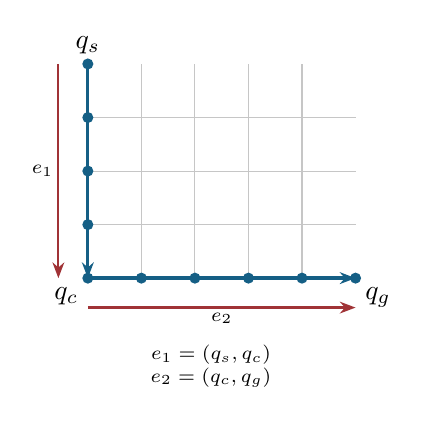
\begin{tikzpicture}[x=.68cm,y=.68cm]
\foreach \y in {1,2,3}{\draw[gray!45] (0,\y)--(5,\y);}
\foreach \x in {1,2,3,4}{\draw[gray!45] (\x,0)--(\x,4);}
\draw[flow,very thick] (0,4)--(0,0);
\draw[flow,very thick] (0,0)--(5,0);
\foreach \y in {0,1,2,3,4}{\fill[accent] (0,\y) circle (2pt);}
\foreach \x in {1,2,3,4,5}{\fill[accent] (\x,0) circle (2pt);}
\node[above] at (0,4) {$q_s$};
\node[below left] at (0,0) {$q_c$};
\node[below right] at (5,0) {$q_g$};
\draw[flow,draw=collision,thick] (-.55,4)--node[lab,left] {$e_1$}(-.55,0);
\draw[flow,draw=collision,thick] (0,-.55)--node[lab,below] {$e_2$}(5,-.55);
\node[align=center,font=\scriptsize] at (2.3,-1.65) {$e_1=(q_s,q_c)$\\$e_2=(q_c,q_g)$};
\end{tikzpicture}

\end{center}
\end{column}
\begin{column}{.62\textwidth}
\footnotesize $q_s\to q_c$, $q_c\to q_g$의 두 직선 Direct Edge를 추가한다. 기존 격자 엣지를 포함한 모든 엣지에 모션 프로파일의 주행시간을 부여한다.
\[
w(e)=\mathcal T_{\rm motion}
       (d_e;\,v_e^{\rm in},v_e^{\rm out},a,b,v_{\max})
\]
\[
w(e_1)=\mathcal T(d_1;0,0),\qquad
w(e_2)=\mathcal T(d_2;0,0)
\]
\[
C_{\rm turn}(e_i,e_{i+1})=
\frac{|\Delta\theta(e_i,e_{i+1})|}{\omega},
\quad |\Delta\theta|\in\{0^\circ,90^\circ,180^\circ\}.
\]
\[
\boxed{C(P)=\sum_{e\in P}w(e)+
\sum_{(e_i,e_{i+1})\in P}C_{\rm turn}(e_i,e_{i+1})}
\]
\[
d_1=d_2=6\,{\rm m}:\quad
7.651+\frac{90^\circ}{45^\circ/{\rm s}}+7.651
=17.302\,{\rm s}.
\]
\end{column}
\end{columns}
\medskip
\footnotesize $d_e$는 엣지 길이, $v_e^{\rm in},v_e^{\rm out}$는 양 끝 속도, $\theta_e$는 방향, $\Delta\theta$는 최소 방향 변화각이다. 연속 직진 엣지에서는 속도를 이어가고 회전할 때 정지한다. 탐색 상태는 $(p,\theta,v)$로 두며 Direct Edge 내부 제어점은 보존한다. $P$는 후보 경로, $d_1,d_2$는 두 Direct Edge의 길이다. $\mathcal T_{\rm motion}$은 프로파일 주행시간[s]이며 $\mathcal T(d;0,0)$은 4장의 정지-정지 주행시간이다.
\end{frame}

\begin{frame}{제어점을 통과하는 Direct Edge의 개수}
\begin{columns}[T,onlytextwidth]
\begin{column}{.40\textwidth}
\begin{center}

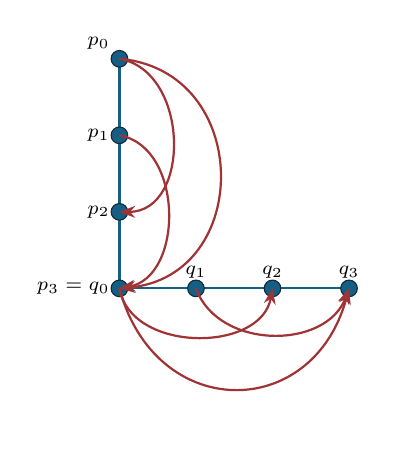
\begin{tikzpicture}[x=.54cm,y=.54cm]
\draw[accent,thick] (0,5.4)--(0,0)--(5.4,0);
\foreach \y in {0,1.8,3.6,5.4}{\filldraw[fill=accent,draw=ink] (0,\y) circle(3pt);}
\foreach \x in {1.8,3.6,5.4}{\filldraw[fill=accent,draw=ink] (\x,0) circle(3pt);}
\draw[flow,draw=collision] (0,5.4) to[out=-10,in=0,looseness=1.2] (0,1.8);
\draw[flow,draw=collision] (0,5.4) to[out=-5,in=5,looseness=1.5] (0,0);
\draw[flow,draw=collision] (0,3.6) to[out=-10,in=10,looseness=1.1] (0,0);
\draw[flow,draw=collision] (0,0) to[out=-80,in=-100,looseness=1.1] (3.6,0);
\draw[flow,draw=collision] (0,0) to[out=-75,in=-105,looseness=1.55] (5.4,0);
\draw[flow,draw=collision] (1.8,0) to[out=-70,in=-110,looseness=1.1] (5.4,0);
\node[above left,font=\scriptsize] at (0,5.4) {$p_0$};
\node[left,font=\scriptsize] at (0,3.6) {$p_1$};
\node[left,font=\scriptsize] at (0,1.8) {$p_2$};
\node[left,font=\scriptsize] at (0,0) {$p_3=q_0$};
\node[above,font=\scriptsize] at (1.8,0) {$q_1$};
\node[above,font=\scriptsize] at (3.6,0) {$q_2$};
\node[above,font=\scriptsize] at (5.4,0) {$q_3$};
\end{tikzpicture}

\end{center}
\end{column}
\begin{column}{.58\textwidth}
\small 양 끝을 포함해 한 직선에 제어점이 $n$개 있다고 하자. 한 방향으로 연결 가능한 점 쌍은 $\binom n2$개이며, 그중 $n-1$개는 이미 존재하는 인접 격자 엣지다.
\[
\boxed{E_{\rm add}^{\rightarrow}(n)
=\binom n2-(n-1)=\frac{(n-1)(n-2)}2}
\]
\[
E_{\rm add}^{\leftrightarrow}(n)=(n-1)(n-2).
\]

\begin{center}\small
\begin{tabular}{rrr}\toprule
제어점 $n$ & 한 방향 & 양방향\\\midrule
4 & 3 & 6\\
10 & 36 & 72\\
20 & 171 & 342\\\bottomrule
\end{tabular}\end{center}

\end{column}
\end{columns}
\medskip
\footnotesize 파란 선분은 기존 인접 엣지다. 빨간 곡선은 중간 제어점을 하나 이상 통과하는 직선 주행을 나타낸다. 그림은 직선마다 3개, 표시된 방향으로 총 6개다. 역방향까지 추가하면 12개다.\par\smallskip 현재 제어점 $4\times4$ 격자는 직선이 8개이므로 $8\times6=48$개 directed edge를 추가한다. 기존 48개와 합하면 총 96개다.
\end{frame}

\begin{frame}[plain]
\centering
{\color{accent}\LARGE Part 2\par}\vspace{8mm}
{\LARGE Traffic Management\par}
\end{frame}

\begin{frame}{정의 1: 경로와 부분 경로}
\small 간섭 회피에서는 \textbf{시간을 추상화하되 경로의 진행 순서와 단계 사이의 선후관계를 유지}한다. 수치적인 시각·속도는 이후 실제 운동과 성능 평가에서 다룬다.
\medskip\par
\normalsize 이동물체 $i$의 경로는 시작 상태부터 끝 상태까지의 연속 경로이다.
\begin{equation}
P_i:[0,1]\longrightarrow\mathcal Q_i,\qquad p_i^s=P_i(0),\quad p_i^e=P_i(1).
\tag{1}
\end{equation}
\small $\mathcal Q_i$는 위치·방향 등의 배치 상태 공간이며, $u\in[0,1]$은 \textbf{시간이 아닌 경로 진행값}이다.
\medskip\par
\normalsize $0\le a\le b\le1$일 때, 원래 순서대로 $P_i(a)$부터 $P_i(b)$까지 따라가는 부분을 부분 경로라 한다.
\begin{equation}
P_i^{[a,b]}:=P_i\big|_{[a,b]}.
\tag{2}
\end{equation}
\small 같은 공간 위치를 다시 지나더라도 경로 진행값으로 서로 다른 경유를 구별한다.
\end{frame}

\begin{frame}{정의 2: 점유 영역과 부분 경로의 Sweep}
경로 상태 $P_i(u)$에서 이동물체가 차지하는 영역을 $B_i(u)$라 한다.
\begin{equation}B_i(u)\subseteq\mathbb R^d,\qquad u\in[0,1].\tag{3}\end{equation}
부분 경로의 sweep은 그 구간에서 점유하는 모든 영역의 합집합이다.
\begin{equation}S_i(P_i^{[a,b]}):=\bigcup_{u\in[a,b]}B_i(u).\tag{4}\end{equation}
\begin{center}
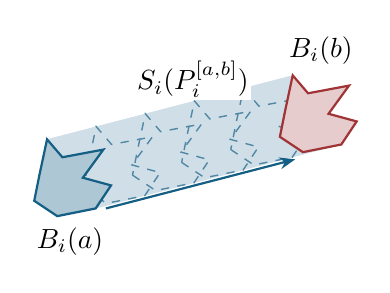
\begin{tikzpicture}[scale=.65]
\path[fill=accent!20,draw=none] (-0.8000,-0.3500)--(-0.3500,-0.6500)--(0.4000,-0.5000)--(0.7000,-0.0500)--(0.1500,0.1000)--(0.5500,0.6500)--(-0.2500,0.5000)--(-0.5500,0.8500)--(-0.7000,0.1500)--cycle;
\path[fill=accent!20,draw=none] (4.0000,0.9000)--(4.4500,0.6000)--(5.2000,0.7500)--(5.5000,1.2000)--(4.9500,1.3500)--(5.3500,1.9000)--(4.5500,1.7500)--(4.2500,2.1000)--(4.1000,1.4000)--cycle;
\path[fill=accent!20,draw=none] (-0.8000,-0.3500)--(-0.3500,-0.6500)--(4.4500,0.6000)--(4.0000,0.9000)--cycle;
\path[fill=accent!20,draw=none] (-0.3500,-0.6500)--(0.4000,-0.5000)--(5.2000,0.7500)--(4.4500,0.6000)--cycle;
\path[fill=accent!20,draw=none] (0.4000,-0.5000)--(0.7000,-0.0500)--(5.5000,1.2000)--(5.2000,0.7500)--cycle;
\path[fill=accent!20,draw=none] (0.7000,-0.0500)--(0.1500,0.1000)--(4.9500,1.3500)--(5.5000,1.2000)--cycle;
\path[fill=accent!20,draw=none] (0.1500,0.1000)--(0.5500,0.6500)--(5.3500,1.9000)--(4.9500,1.3500)--cycle;
\path[fill=accent!20,draw=none] (0.5500,0.6500)--(-0.2500,0.5000)--(4.5500,1.7500)--(5.3500,1.9000)--cycle;
\path[fill=accent!20,draw=none] (-0.2500,0.5000)--(-0.5500,0.8500)--(4.2500,2.1000)--(4.5500,1.7500)--cycle;
\path[fill=accent!20,draw=none] (-0.5500,0.8500)--(-0.7000,0.1500)--(4.1000,1.4000)--(4.2500,2.1000)--cycle;
\path[fill=accent!20,draw=none] (-0.7000,0.1500)--(-0.8000,-0.3500)--(4.0000,0.9000)--(4.1000,1.4000)--cycle;
\begin{scope}[shift={(0.960,0.250)}]\draw[accent!75,dashed,line width=.5pt] (-0.8000,-0.3500)--(-0.3500,-0.6500)--(0.4000,-0.5000)--(0.7000,-0.0500)--(0.1500,0.1000)--(0.5500,0.6500)--(-0.2500,0.5000)--(-0.5500,0.8500)--(-0.7000,0.1500)--cycle;\end{scope}
\begin{scope}[shift={(1.920,0.500)}]\draw[accent!75,dashed,line width=.5pt] (-0.8000,-0.3500)--(-0.3500,-0.6500)--(0.4000,-0.5000)--(0.7000,-0.0500)--(0.1500,0.1000)--(0.5500,0.6500)--(-0.2500,0.5000)--(-0.5500,0.8500)--(-0.7000,0.1500)--cycle;\end{scope}
\begin{scope}[shift={(2.880,0.750)}]\draw[accent!75,dashed,line width=.5pt] (-0.8000,-0.3500)--(-0.3500,-0.6500)--(0.4000,-0.5000)--(0.7000,-0.0500)--(0.1500,0.1000)--(0.5500,0.6500)--(-0.2500,0.5000)--(-0.5500,0.8500)--(-0.7000,0.1500)--cycle;\end{scope}
\begin{scope}[shift={(3.840,1.000)}]\draw[accent!75,dashed,line width=.5pt] (-0.8000,-0.3500)--(-0.3500,-0.6500)--(0.4000,-0.5000)--(0.7000,-0.0500)--(0.1500,0.1000)--(0.5500,0.6500)--(-0.2500,0.5000)--(-0.5500,0.8500)--(-0.7000,0.1500)--cycle;\end{scope}
\path[fill=accent!35,draw=accent,thick] (-0.8000,-0.3500)--(-0.3500,-0.6500)--(0.4000,-0.5000)--(0.7000,-0.0500)--(0.1500,0.1000)--(0.5500,0.6500)--(-0.2500,0.5000)--(-0.5500,0.8500)--(-0.7000,0.1500)--cycle;
\begin{scope}[shift={(4.8,1.25)}]\path[fill=collision!25,draw=collision,thick] (-0.8000,-0.3500)--(-0.3500,-0.6500)--(0.4000,-0.5000)--(0.7000,-0.0500)--(0.1500,0.1000)--(0.5500,0.6500)--(-0.2500,0.5000)--(-0.5500,0.8500)--(-0.7000,0.1500)--cycle;\end{scope}
\draw[flow] (.6,-.5)--(4.3,.46);
\node[below] at (-.1,-.68) {$B_i(a)$};
\node[above] at (4.8,2.12) {$B_i(b)$};
\node[above,fill=white,inner sep=1pt] at (2.3,1.6) {$S_i(P_i^{[a,b]})$};
\end{tikzpicture}
\end{center}
\small 그림은 비정형 다각형의 대각선 이동이다. 전체 sweep은 $a=0,b=1$인 같은 연산 $S_i(P_i)$로 나타낸다. 평면은 $d=2$, 공간은 $d=3$이며, 근사 영역을 쓰면 실제 sweep을 포함해야 한다.
\end{frame}

\begin{frame}{예: RMFS의 전체 경로와 부분 경로 Sweep}
\small 랙의 축 정렬 방향은 본체의 회전에도 유지된다. 랙 한 변이 $2L_i$, 중심 위치가 $p_i(u)$이면,
\begin{equation}B_i(u)=p_i(u)+[-L_i,L_i]^2.\tag{5}\end{equation}
\small $P_i^{[a,b]}$가 수평 또는 수직 직선인 경우,
\begin{equation}S_i(P_i^{[a,b]})=[p_i(a),p_i(b)]\oplus[-L_i,L_i]^2.\tag{6}\end{equation}
\begin{columns}[T]
\begin{column}{.49\textwidth}\centering
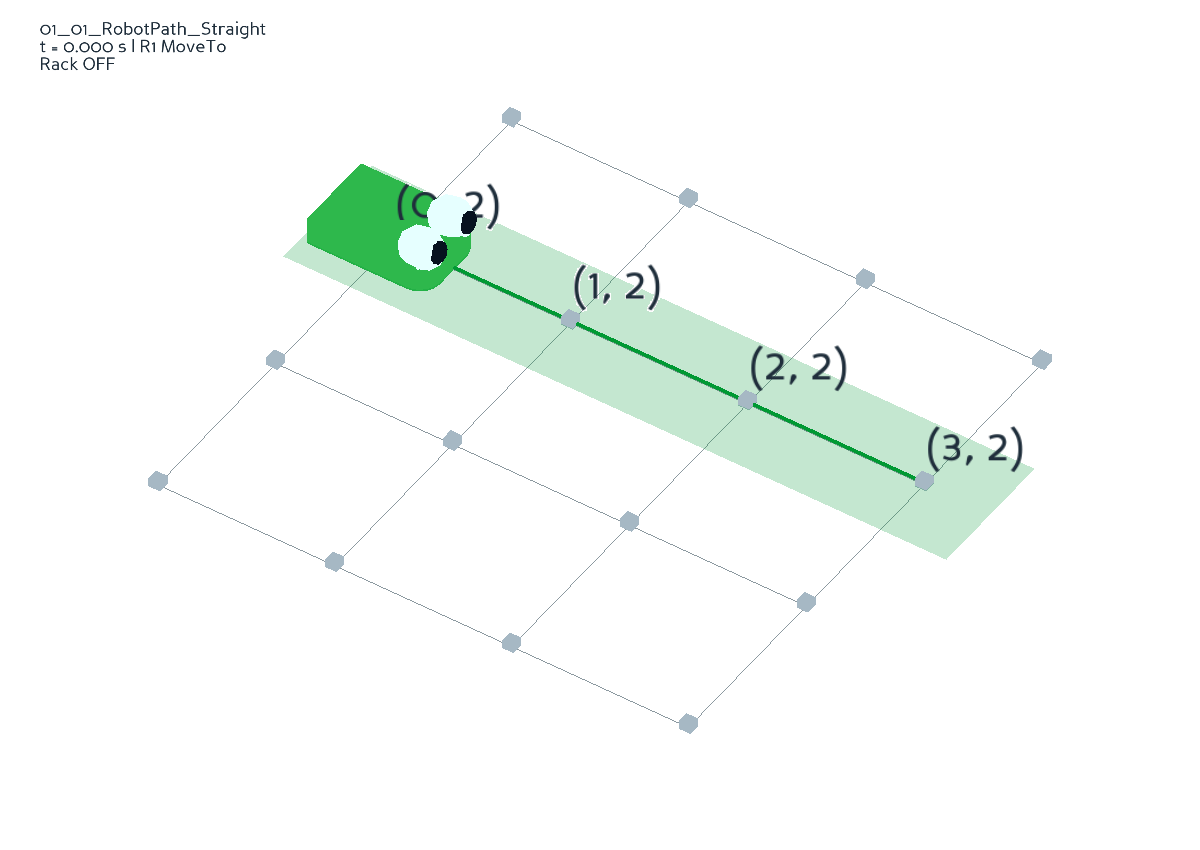
\includegraphics[height=2.65cm,keepaspectratio]{assets/straight_white_sweep.png}\par
{\scriptsize 전체: $(0,2)$부터 $(3,2)$까지.}
\end{column}\begin{column}{.49\textwidth}\centering
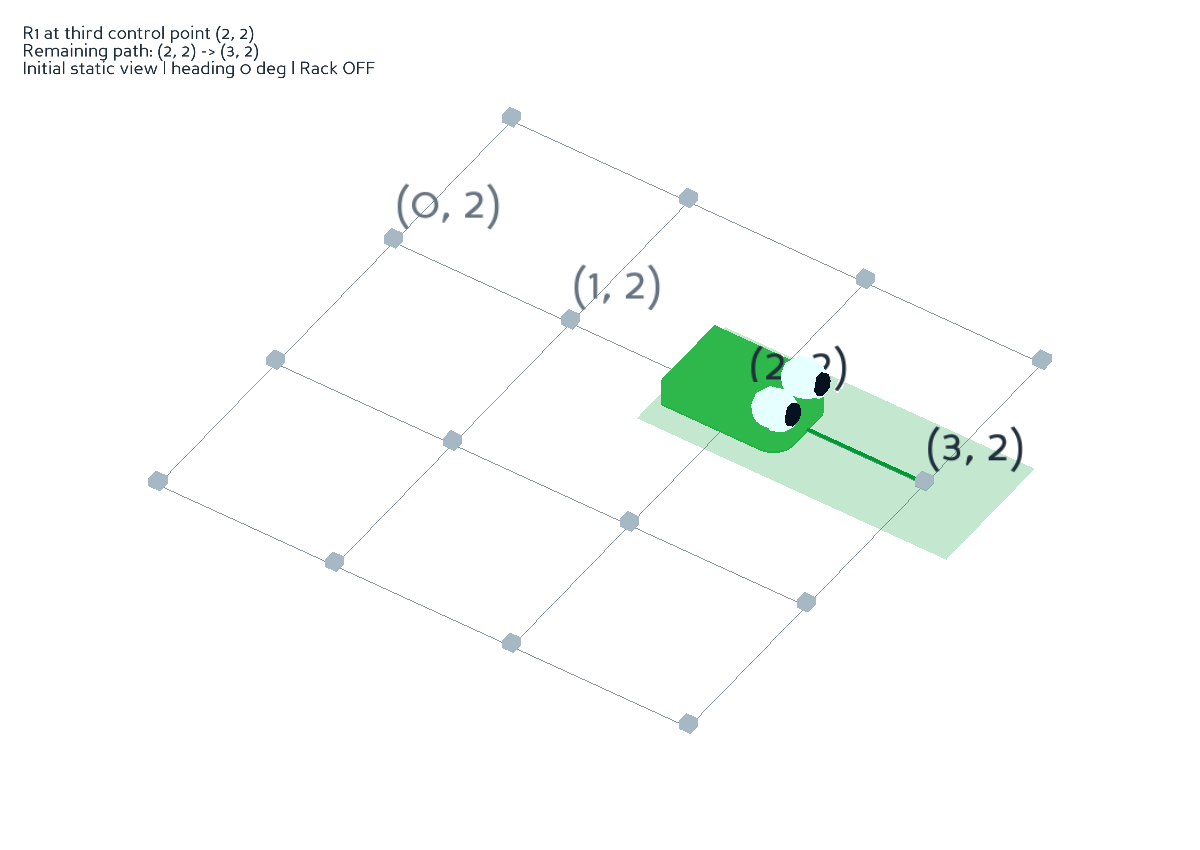
\includegraphics[height=2.65cm,keepaspectratio]{assets/remaining_straight_third_point.png}\par
{\scriptsize 부분: $(2,2)$부터 $(3,2)$까지.}
\end{column}\end{columns}
\small $\oplus$는 Minkowski sum이다. 중심 이동 거리가 $\ell$이면 길이 $\ell+2L_i$, 폭 $2L_i$의 직사각형이며, 양 끝의 점유도 포함한다. 그림 좌표는 제어점 인덱스이다.
\end{frame}

\begin{frame}{정의 3: 점 경로와 대기}
부분 경로의 양 끝 진행값이 같으면 배치 상태가 변하지 않는 \textbf{점 경로}이다. 이를 해당 단계의 대기로 나타낸다.
\begin{equation}
P_i^{[a,a]}:\ \text{상태 }P_i(a)\text{에 대기},\qquad S_i(P_i^{[a,a]})=B_i(a).
\tag{7}
\end{equation}
\begin{center}
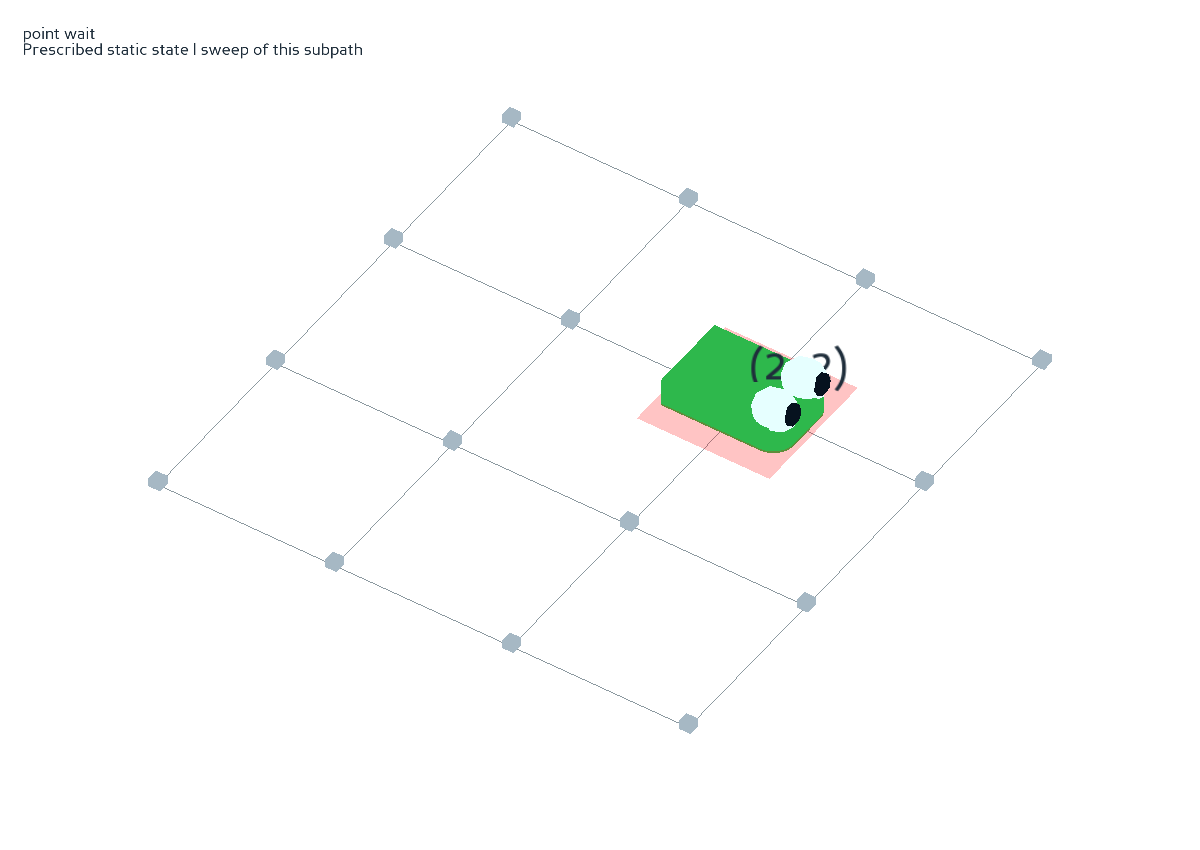
\includegraphics[height=3.0cm,keepaspectratio]{assets/point_wait_white.png}\par
{\scriptsize 제어점 $(2,2)$에 있는 물체의 점 경로 sweep.}
\end{center}
\small 대기는 점유 영역이 없는 상태가 아니다. 이동을 하지 않아도 몸체의 정사각형은 남는다. 따라서 한 물체가 대기하는 경우도 같은 sweep 교차 검사에 포함된다.
\end{frame}

\begin{frame}{정의 4: 대기를 포함한 순서 분할과 연결}
경로를 원래 진행 순서에 따라 유한 개의 부분 경로로 나눈다.
\begin{equation}
0=u_i^0\le\cdots\le u_i^m=1,\qquad P_i^{(k)}:=P_i^{[u_i^{k-1},u_i^k]}.
\tag{8}
\end{equation}
연결 연산 $\circ$로 원래 경로를 복원한다.
\begin{equation}
P_i=P_i^{(1)}\circ\cdots\circ P_i^{(m)},\qquad
P_j=P_j^{(1)}\circ\cdots\circ P_j^{(m)}.
\tag{9}
\end{equation}
\small 필요하면 점 경로의 대기를 넣어 두 경로의 단계 수를 $m$으로 맞춘다. 인접 부분 경로의 끝과 시작은 이어진다.
\medskip\par
\normalsize 연결된 경로의 점유 영역은 부분별 sweep의 합집합이다.
\begin{equation}S_i(P_i)=\bigcup_{k=1}^{m}S_i(P_i^{(k)}).\tag{10}\end{equation}
\small 합집합은 점유 공간만 나타내며, 이동 순서는 식 (9)의 연결에 유지된다. RMFS에서는 각 직선 sweep이 직사각형이므로 전체는 그 합집합이다.
\end{frame}

\begin{frame}{정의 5: 무간섭 부분 경로 짝짓기}
두 물체의 분할을 단계별로 짝짓는다.
\begin{equation}
\left(P_i^{(k)},P_j^{(k)}\right),\qquad k=1,\ldots,m.
\tag{11}
\end{equation}
모든 짝에서 두 부분 경로의 sweep이 교차하지 않으면 \textbf{무간섭 부분 경로 짝짓기}라 한다.
\begin{equation}
S_i(P_i^{(k)})\cap S_j(P_j^{(k)})=\varnothing,\qquad k=1,\ldots,m.
\tag{12}
\end{equation}
\end{frame}

\begin{frame}{예: 전체 경로 간섭을 두 무간섭 짝으로 분해}
\small 전체 경로는 $P_1=[(0,1),(3,1)]$, $P_2=[(1,1),(1,3)]$이다. 두 전체 sweep은 겹치지만, 대기를 넣어 다음 두 짝으로 나눌 수 있다.
\begin{columns}[T]
\begin{column}{.32\textwidth}\centering
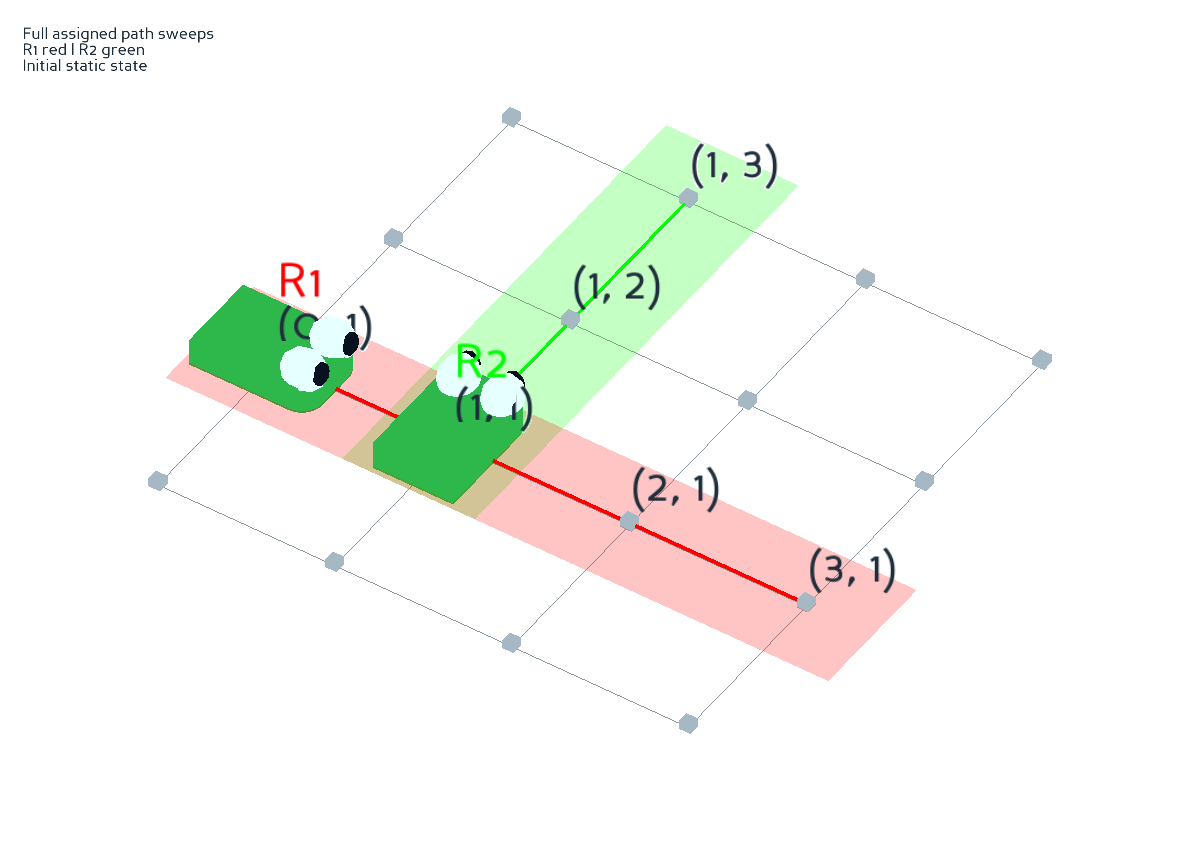
\includegraphics[height=2.6cm,keepaspectratio]{assets/paired_full_white.png}\par
{\scriptsize 전체 경로: sweep이 겹친다.\par $S_1(P_1)\cap S_2(P_2)\ne\varnothing$.}
\end{column}
\begin{column}{.32\textwidth}\centering
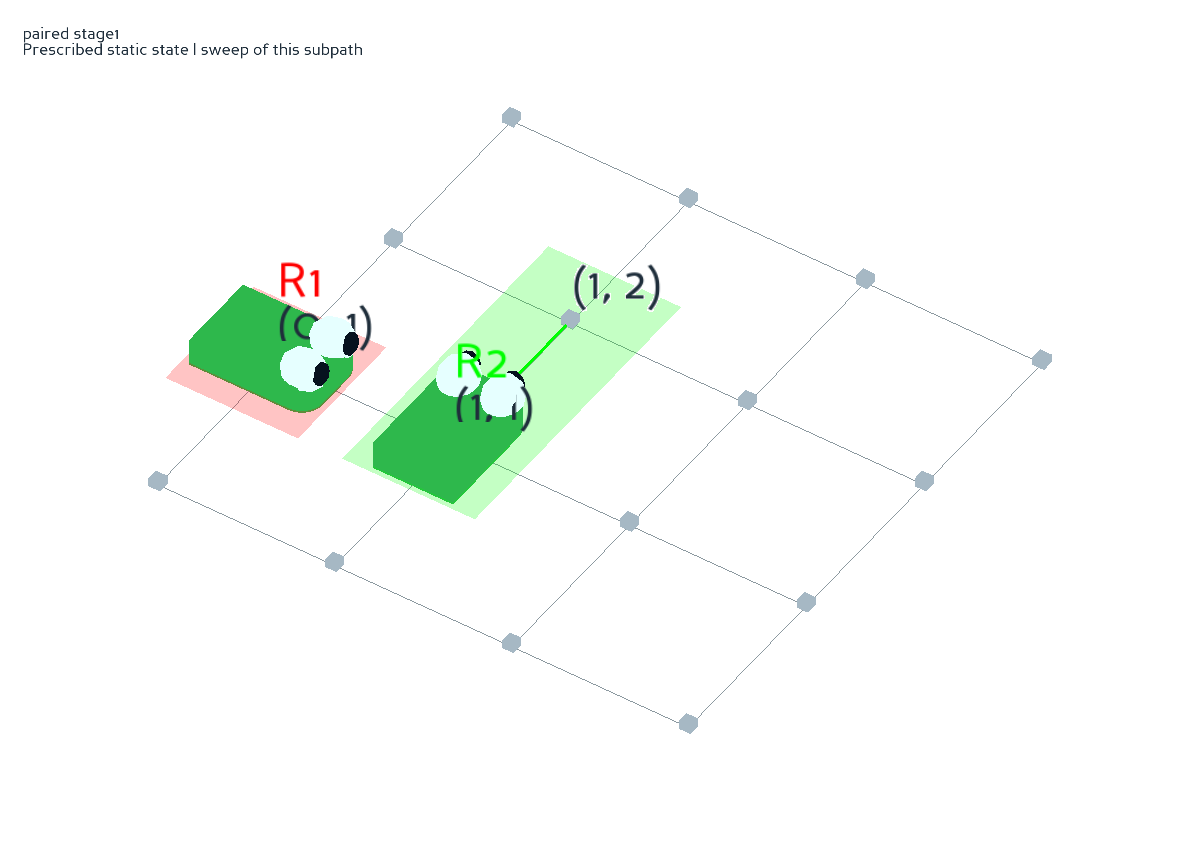
\includegraphics[height=2.6cm,keepaspectratio]{assets/paired_stage1_white.png}\par
{\scriptsize 첫 짝: 빨강은 대기, 초록은 위로.\par 두 부분 경로의 sweep은 분리된다.}
\end{column}
\begin{column}{.32\textwidth}\centering
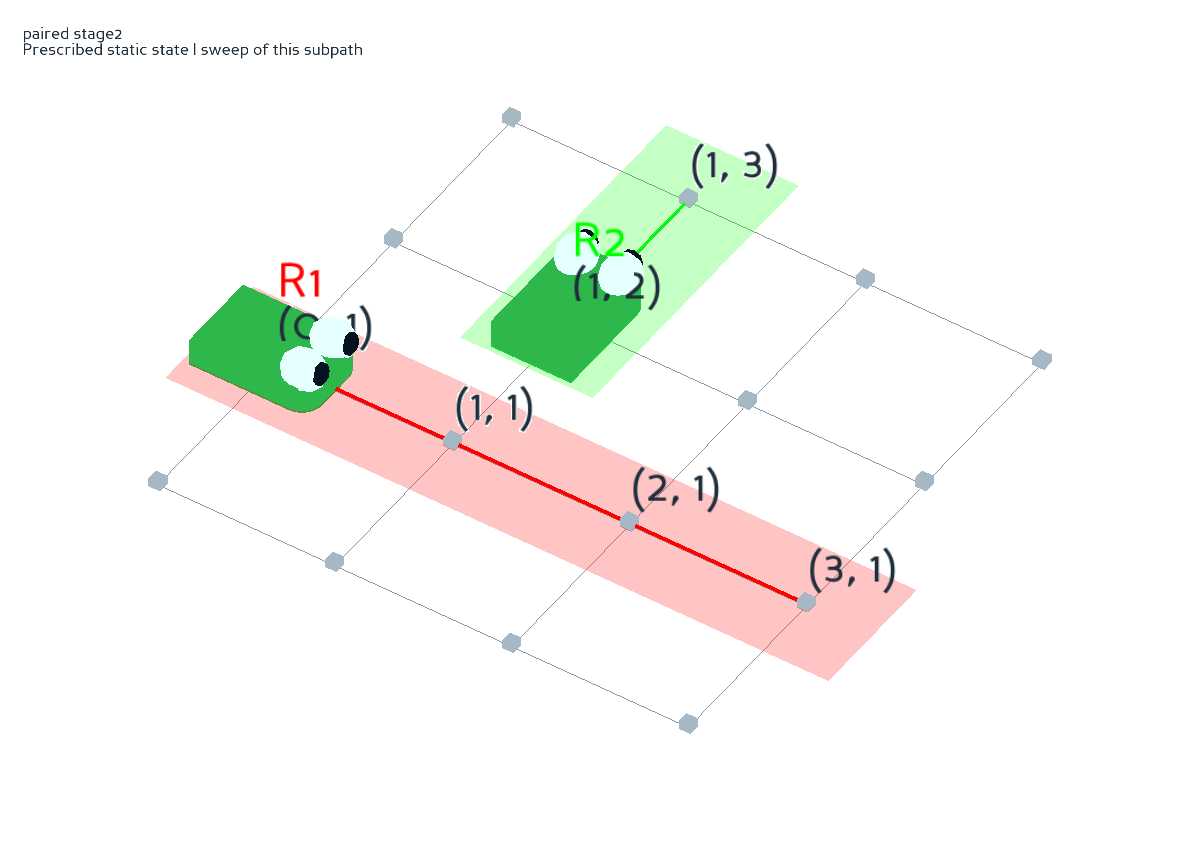
\includegraphics[height=2.6cm,keepaspectratio]{assets/paired_stage2_white.png}\par
{\scriptsize 둘째 짝: 둘 다 남은 부분을 이동.\par 두 부분 경로의 sweep은 분리된다.}
\end{column}\end{columns}
\begin{equation}
\begin{aligned}
P_1^{(1)}&=[(0,1),(0,1)],& P_2^{(1)}&=[(1,1),(1,2)],\\
P_1^{(2)}&=[(0,1),(3,1)],& P_2^{(2)}&=[(1,2),(1,3)].
\end{aligned}
\tag{13}
\end{equation}
\small \textbf{전체 sweep의 교차가 곧 완료 불가능을 뜻하지는 않는다.} 각 짝은 무간섭이고, 부분 경로들을 순서대로 연결하면 원래 두 경로가 된다.
\par\smallskip\scriptsize 02\_09 예제의 초기 배치와 두 부분 경로 짝을 그린 정적 화면. 좌표는 제어점 인덱스이다.
\end{frame}

\begin{frame}{예: 역방향 경로 간섭과 첫 번째 무간섭 짝}
\small 두 물체는 같은 수평 통로를 반대 방향으로 지난다. 출발점과 목적지는 통로 밖에 있다.
\par\smallskip
$P_1:(0,3)\to(0,2)\to(3,2)\to(3,3)$,\par
$P_2:(3,1)\to(3,2)\to(0,2)\to(0,1)$.
\begin{columns}[T]
\begin{column}{.49\textwidth}\centering
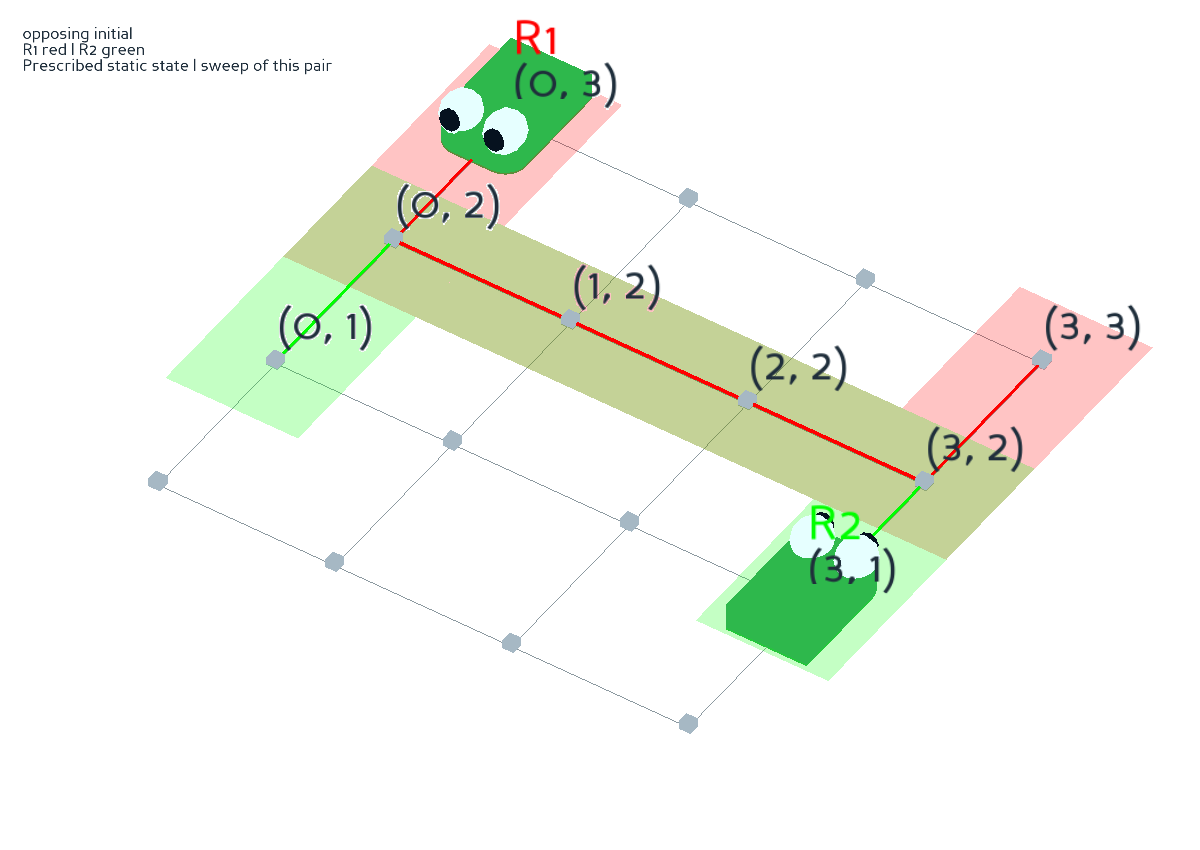
\includegraphics[height=2.8cm,keepaspectratio]{assets/opposing_initial_white.png}\par
{\scriptsize 초기 전체 경로: 빨강·초록 sweep이 겹친다.}
\end{column}\begin{column}{.49\textwidth}\centering
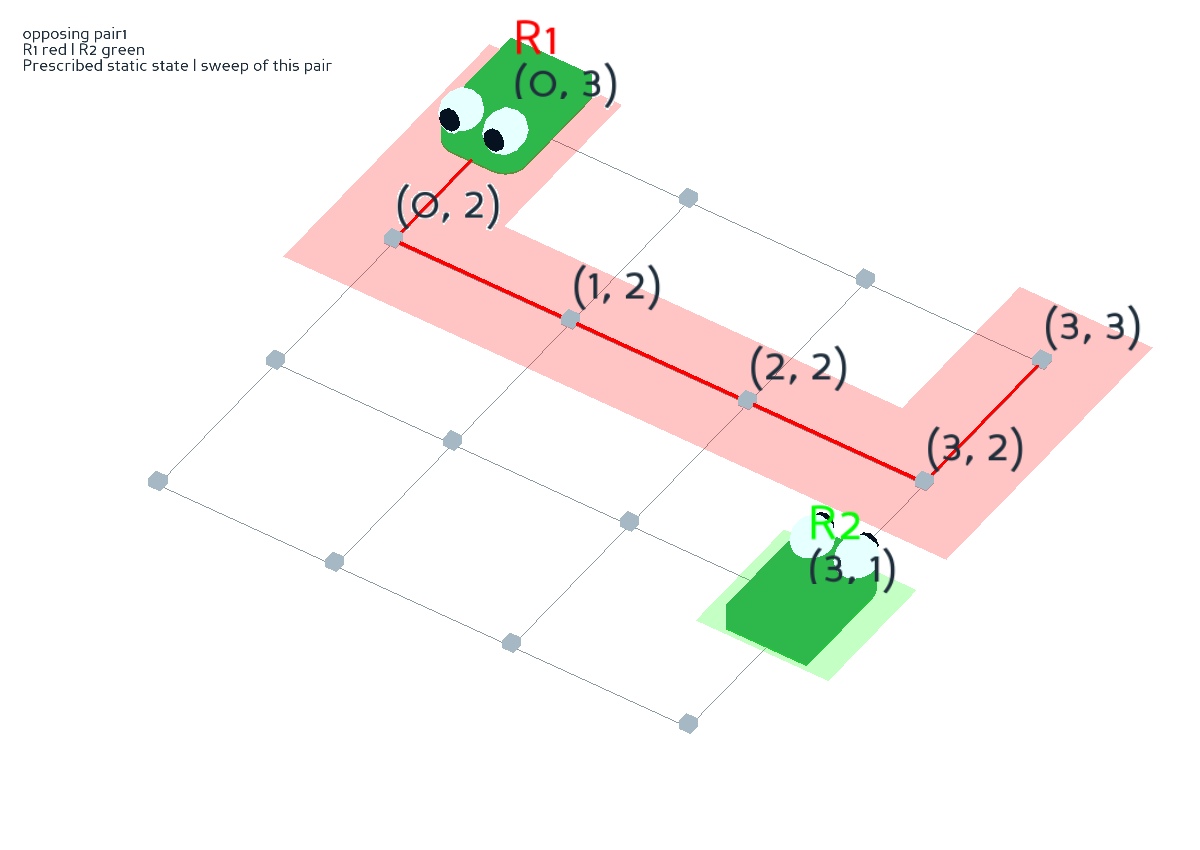
\includegraphics[height=2.8cm,keepaspectratio]{assets/opposing_pair1_white.png}\par
{\scriptsize 첫 짝: 초록은 출발점에 대기, 빨강만 전체 이동.}
\end{column}\end{columns}

\begin{equation}
\begin{aligned}
&P_1^{(1)}=P_1,\qquad P_2^{(1)}=[(3,1),(3,1)],\\
&S_1(P_1^{(1)})\cap S_2(P_2^{(1)})=\varnothing.
\end{aligned}
\tag{13a}
\end{equation}
\small 초록의 대기는 출발점의 몸체 영역을 남긴다. 이 정사각형은 빨강의 전체 sweep과 겹치지 않으므로, 빨강은 통로를 지나 목적지 $(3,3)$까지 빠져나갈 수 있다.
\par\smallskip\scriptsize 02\_07 예제 경로를 두 짝으로 분할한 정적 예시. 좌표는 제어점 인덱스이다.
\end{frame}

\begin{frame}{예: 역방향 간섭의 두 번째 짝과 전체 완료}
\begin{columns}[T]
\begin{column}{.49\textwidth}\centering
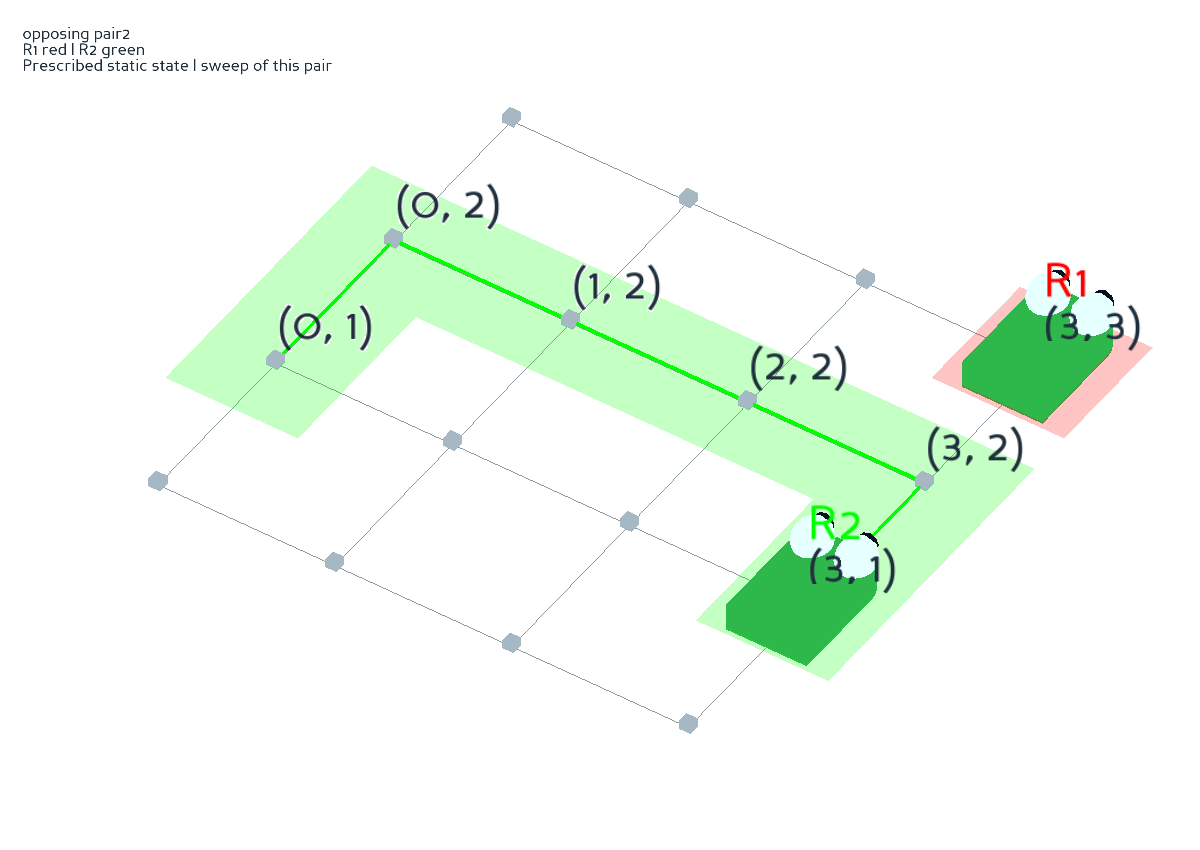
\includegraphics[height=2.8cm,keepaspectratio]{assets/opposing_pair2_white.png}\par
{\scriptsize 둘째 짝: 빨강은 목적지에 대기, 초록만 전체 이동.}
\end{column}\begin{column}{.49\textwidth}\centering
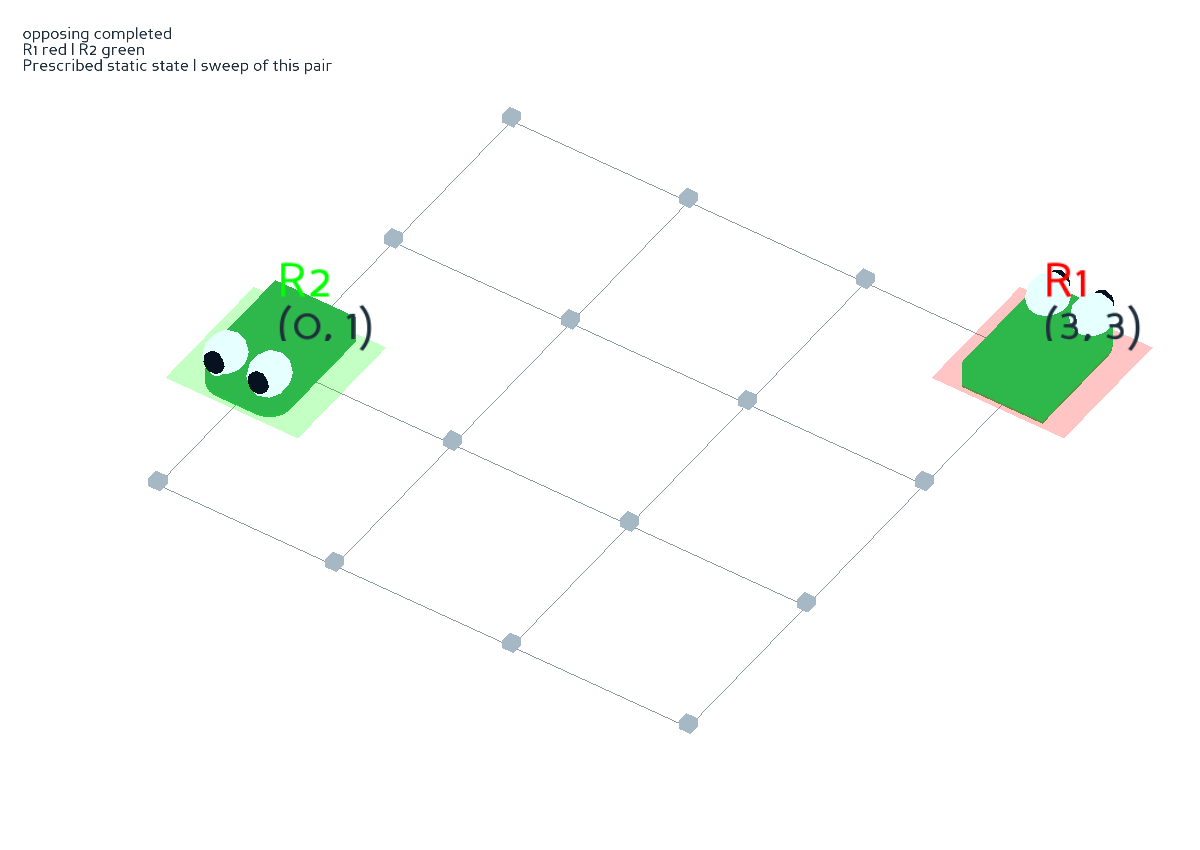
\includegraphics[height=2.8cm,keepaspectratio]{assets/opposing_completed_white.png}\par
{\scriptsize 두 짝의 실행 후: 두 물체 모두 목적지에 도착.}
\end{column}\end{columns}

\begin{equation}
\begin{aligned}
&P_1^{(2)}=[(3,3),(3,3)],\qquad P_2^{(2)}=P_2,\\
&S_1(P_1^{(2)})\cap S_2(P_2^{(2)})=\varnothing.
\end{aligned}
\tag{13b}
\end{equation}
\small 빨강의 목적지 점유 영역은 초록의 sweep과 겹치지 않는다. 초록은 반대 방향으로 통로를 지나 목적지 $(0,1)$까지 이동한다.
\medskip\par
\textbf{전체 경로끼리는 간섭하지만, 대기를 포함한 두 짝은 각각 무간섭이다.} 첫 짝을 완료한 뒤 둘째 짝을 실행하면 전체 경로를 완료한다.
\par\smallskip\scriptsize 수치적인 이동 시각이나 속도를 정하지 않고, 부분 경로 짝의 순서와 공간 점유만으로 설명한다. 그림은 지정한 정지 상태이며 자동 제어 실행 기록은 아니다.
\end{frame}

\begin{frame}{반례: 마주 보는 두 물체는 끝까지 짝지을 수 없다}
\small 두 물체가 같은 직선 경로의 양 끝에서 출발하여 서로의 출발점을 목적지로 가진다. 경로는 고정하며, 우회하여 비켜설 공간은 사용하지 않는다.
\begin{center}
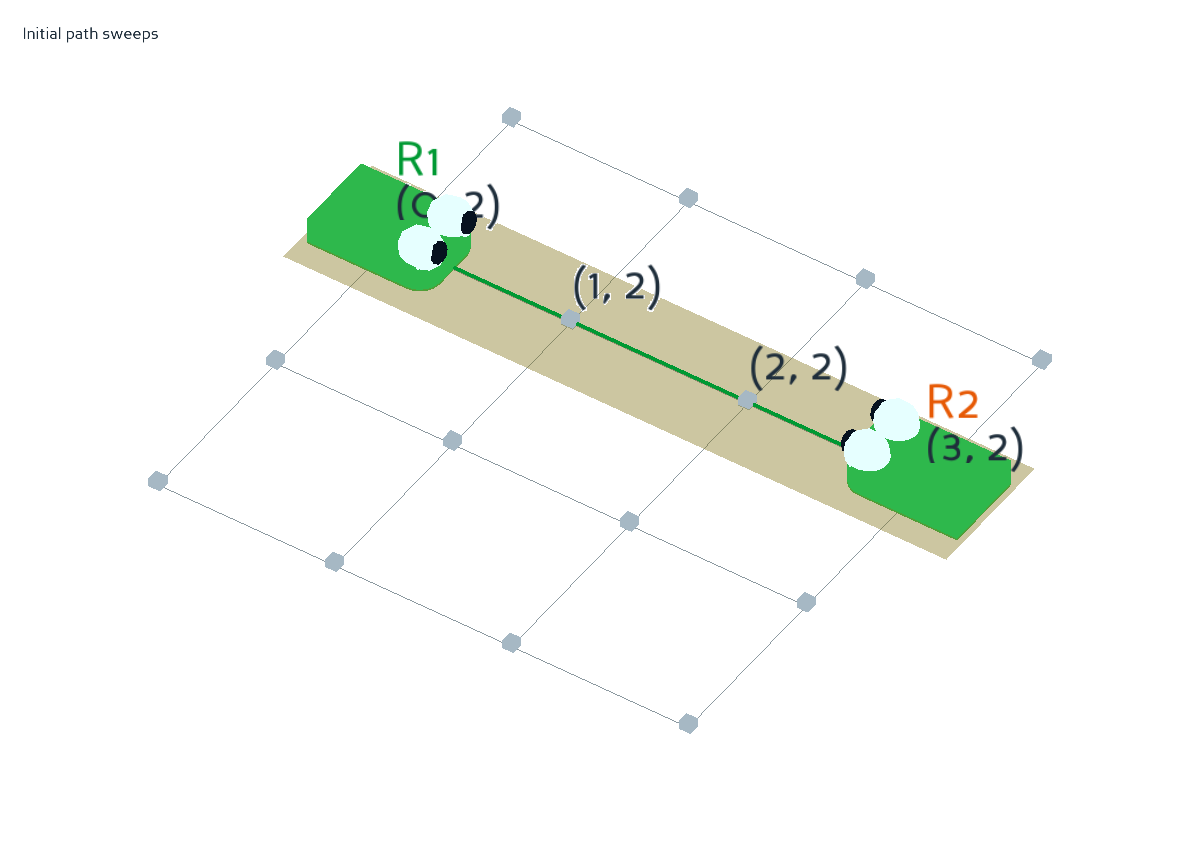
\includegraphics[height=3.0cm,keepaspectratio]{assets/p25_initial_white.png}\par
{\scriptsize $P_1:[(0,2),(3,2)]$,\quad $P_2:[(3,2),(0,2)]$. 전체 sweep이 겹친다.}
\end{center}
\small 경로 진행 중 두 물체는 항상 같은 직선 위에 있다. 출발과 도착에서 중심의 좌우 순서는 반대이다.
\begin{equation}
x_1^s<x_2^s,\qquad x_1^e>x_2^e.
\tag{13c}
\end{equation}
\small 연속적으로 이동하면서 이 순서를 뒤집으려면 두 몸체가 만나야 한다. 따라서 대기를 넣거나 먼저 보낼 물체를 바꿔도, 두 전체 경로를 끝까지 구성하는 \textbf{유한한 무간섭 부분 경로 짝짓기는 존재하지 않는다.}
\par\smallskip{\tiny\texttt{\detokenize{python -m examples.RMFS.Tests.02_05_RobotPath_OppositeDirection_Collision --white-background}}}
\end{frame}

\begin{frame}{정리 1: 비 교차 Sweep 짝짓기에 의한 안전한 완료}
\textbf{정리 1.} 두 이동물체의 전체 경로가 유한 개의 무간섭 부분 경로 짝으로 연결되고, 각 짝의 실행에 유한한 시간이 소요된다면, \textbf{그 짝들을 순서대로 실행하면 유한한 시간에 충돌 없이 전체 경로를 완료할 수 있다.}
\medskip\par
\textbf{증명.} 각 짝의 두 sweep은 교차하지 않으며, 이동 중이거나 끝점에서 대기 중인 물체의 점유 영역은 자기 sweep에 포함된다. 따라서 각 짝의 실행은 충돌 없이 이루어진다.
\medskip\par
각 짝을 완료한 뒤 다음 짝을 실행하므로 전체 실행에서도 충돌하지 않는다. 또한 짝의 개수와 각 짝의 실행시간이 모두 유한하므로 전체 실행시간도 유한하다.
\medskip\par
부분 경로들을 순서대로 연결하면 전체 경로가 되므로 두 물체는 각 목적지에 \textbf{유한시간 내에} 도달한다.\hfill$\square$
\end{frame}

\begin{frame}{정리 1을 세 이동물체에 적용하는 조건}
세 경로를 \textbf{공통된 단계 수 $m$}으로 나누고, 각 단계에서 세 부분 경로를 하나의 묶음으로 둔다.
\[
\left(P_1^{(k)},P_2^{(k)},P_3^{(k)}\right),\qquad k=1,\ldots,m.
\]
각 묶음의 모든 물체 쌍이 무간섭이어야 한다.
\begin{equation}
S_r(P_r^{(k)})\cap S_s(P_s^{(k)})=\varnothing,
\quad 1\le r<s\le3,\quad k=1,\ldots,m.
\tag{14}
\end{equation}
\textbf{따름 성질.} 각 묶음의 실행시간이 유한하면, 묶음들을 순서대로 실행하여 세 경로를 유한시간에 충돌 없이 완료할 수 있다.
\medskip\par
\small \textbf{근거:} 같은 $k$에서 정리 1의 sweep 포함 논리를 세 물체 쌍 모두에 적용한다. 어느 두 몸체도 만나지 않으므로 세 물체 전체가 안전하다. 유한 개 묶음의 연결은 전체 경로를 완료한다.
\medskip\par
\textbf{주의:} 물체 쌍마다 서로 다른 순서로 풀리는 것만으로는 부족하다. 세 물체가 함께 따를 \textbf{하나의 공통 단계 분할}이 필요하다.
\end{frame}

\begin{frame}{풀리는 예: 초기 전체 Sweep은 서로 간섭한다}
\begin{columns}[T]
\begin{column}{.51\textwidth}\centering
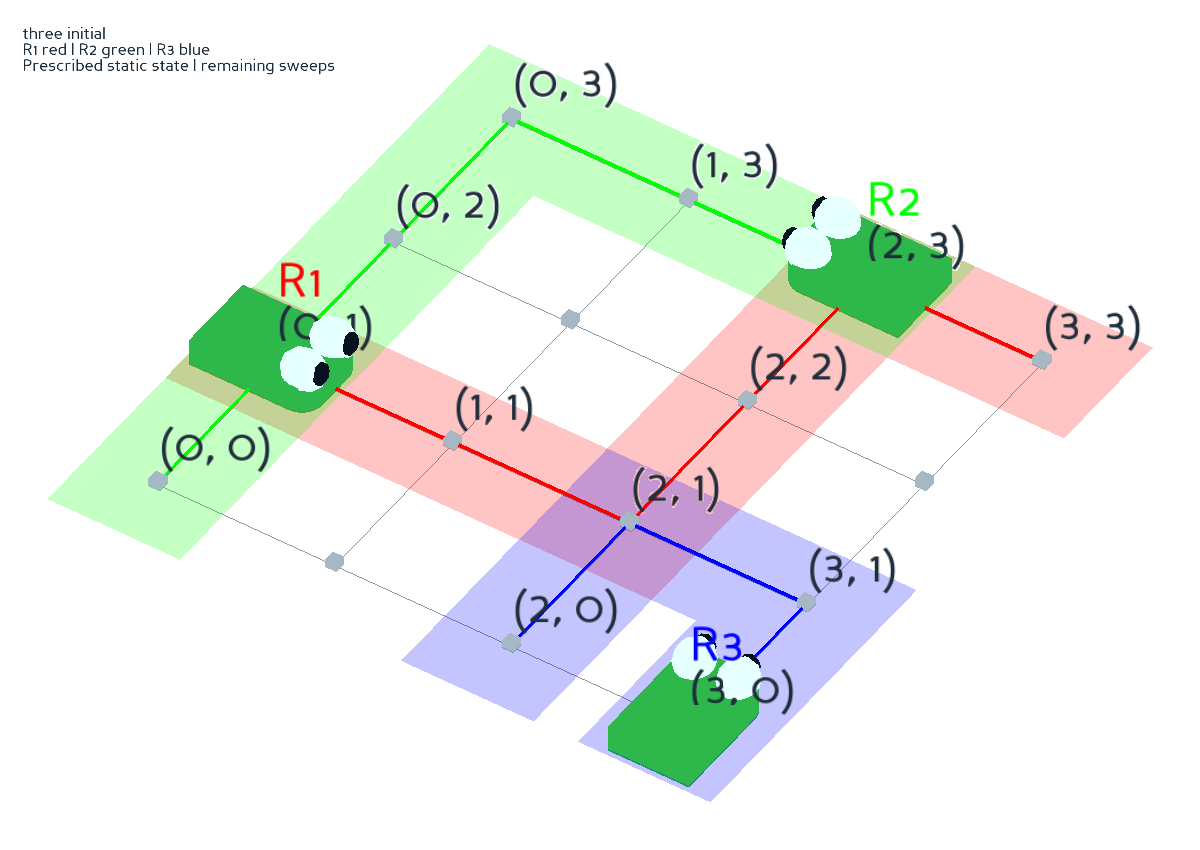
\includegraphics[height=3.65cm,keepaspectratio]{assets/three_initial_white.png}
\end{column}\begin{column}{.47\textwidth}\small
\textbf{03\_04 예제의 세 고정 경로}
\[
\begin{aligned}
P_1:\ &(0,1)\to(2,1)\\
&\to(2,3)\to(3,3),\\
P_2:\ &(2,3)\to(0,3)\to(0,0),\\
P_3:\ &(3,0)\to(3,1)\\
&\to(2,1)\to(2,0).
\end{aligned}
\]
빨강은 초록·파랑과 각각 겹친다. 초록과 파랑은 겹치지 않는다. 세 물체 모두의 경로를 고려해 다음 세 묶음을 구성한다.
\end{column}\end{columns}
\small 모든 그림에서 빨강은 물체 1, 초록은 물체 2, 파랑은 물체 3이다. 좌표는 제어점 인덱스이며, 단계별 그림은 해당 부분 경로의 sweep만 표시한다.
\par\smallskip{\tiny\texttt{\detokenize{python -m examples.RMFS.Tests.03_04_RobotPath_SweepInterference --white-background}}}
\end{frame}

\begin{frame}{첫 묶음: 빨강·초록은 대기하고 파랑이 빠져나간다}
\begin{columns}[T]
\begin{column}{.49\textwidth}\centering
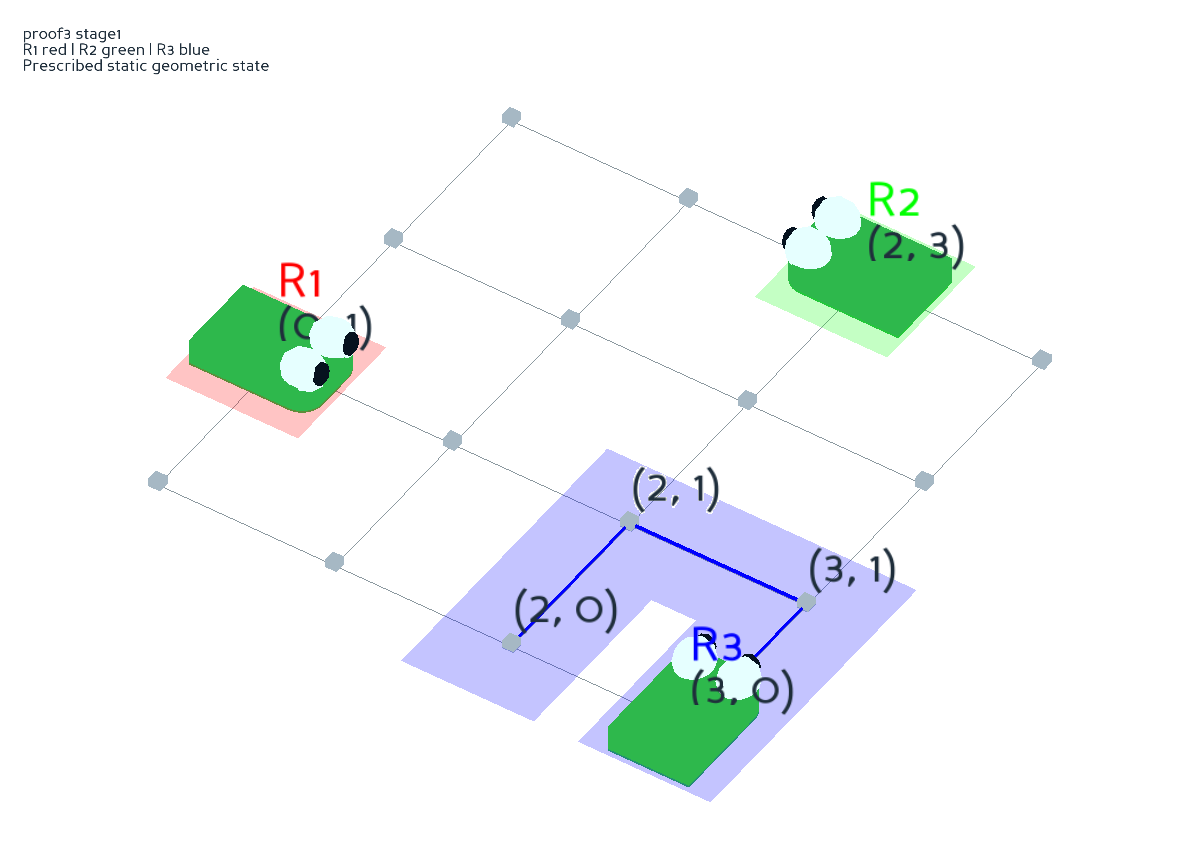
\includegraphics[height=2.65cm,keepaspectratio]{assets/proof3_stage1_white.png}\par{\scriptsize 이번 묶음: 두 점 경로와 파랑의 전체 경로.}
\end{column}\begin{column}{.49\textwidth}\centering
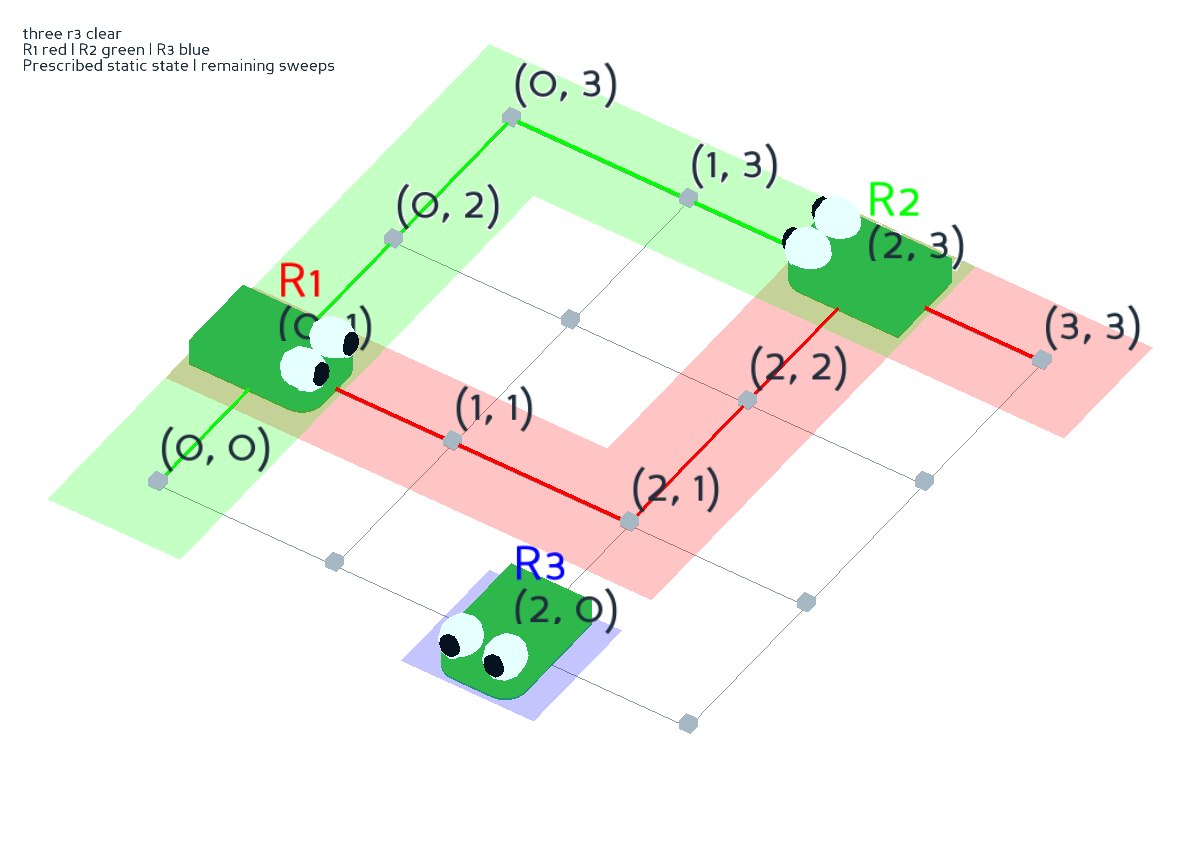
\includegraphics[height=2.65cm,keepaspectratio]{assets/three_r3_clear_white.png}\par{\scriptsize 묶음 완료 후 잔여 경로: 빨강·초록 간섭은 남는다.}
\end{column}\end{columns}

\begin{equation}
\begin{aligned}
P_1^{(1)}&=[(0,1),(0,1)],\\
P_2^{(1)}&=[(2,3),(2,3)],\qquad P_3^{(1)}=P_3.
\end{aligned}
\tag{15}
\end{equation}
\small 왼쪽에서 파란 sweep은 빨강·초록의 현재 몸체 영역과 교차하지 않는다. 두 대기 물체도 서로 떨어져 있으므로 세 쌍이 모두 무간섭이다.
\medskip\par
파랑은 $(2,0)$에 도착해 점유 정사각형만 남는다. 오른쪽의 빨강·초록 잔여 sweep은 아직 겹치지만, 다음 묶음에서 이를 풀 수 있다.
\end{frame}

\begin{frame}{둘째·셋째 묶음: 남은 두 물체의 부분 경로를 연결한다}
\begin{columns}[T]
\begin{column}{.49\textwidth}\centering
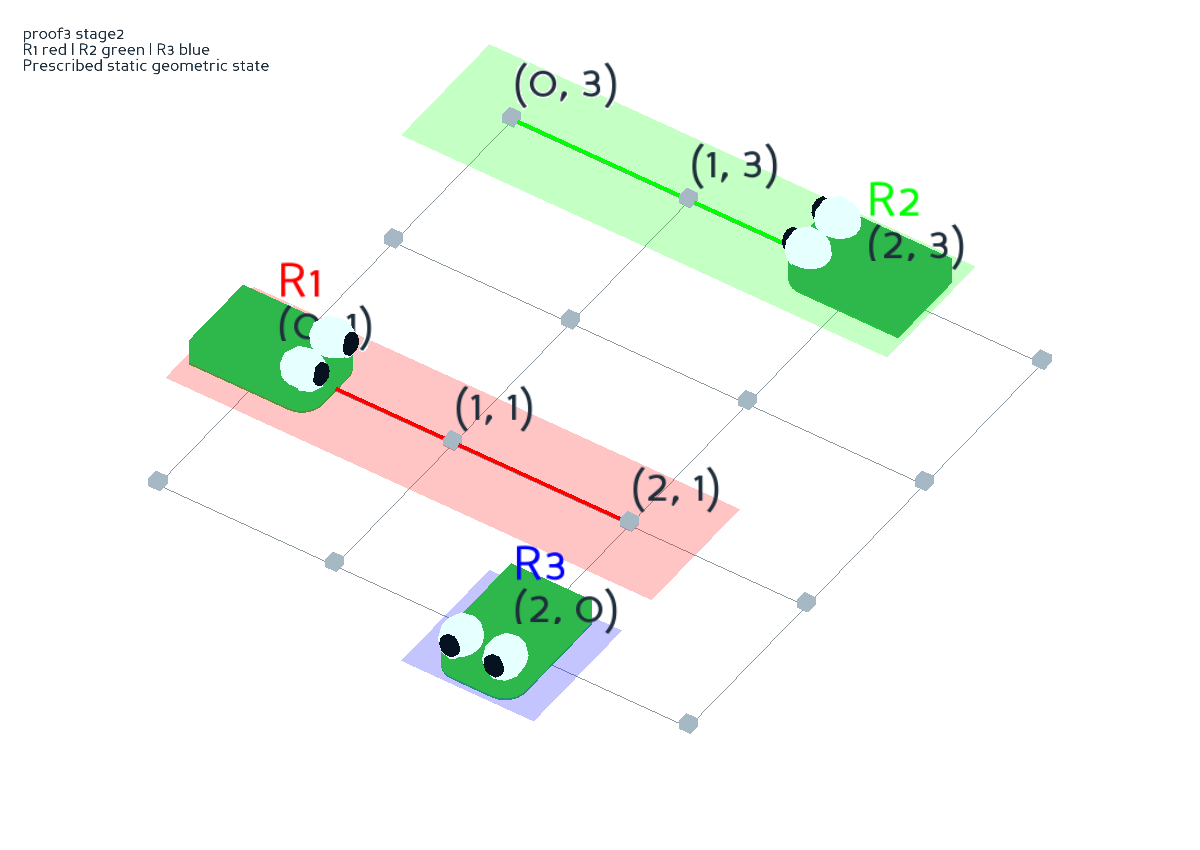
\includegraphics[height=2.65cm,keepaspectratio]{assets/proof3_stage2_white.png}\par{\scriptsize 둘째 묶음: 빨강·초록이 일부 전진, 파랑은 대기.}
\end{column}\begin{column}{.49\textwidth}\centering
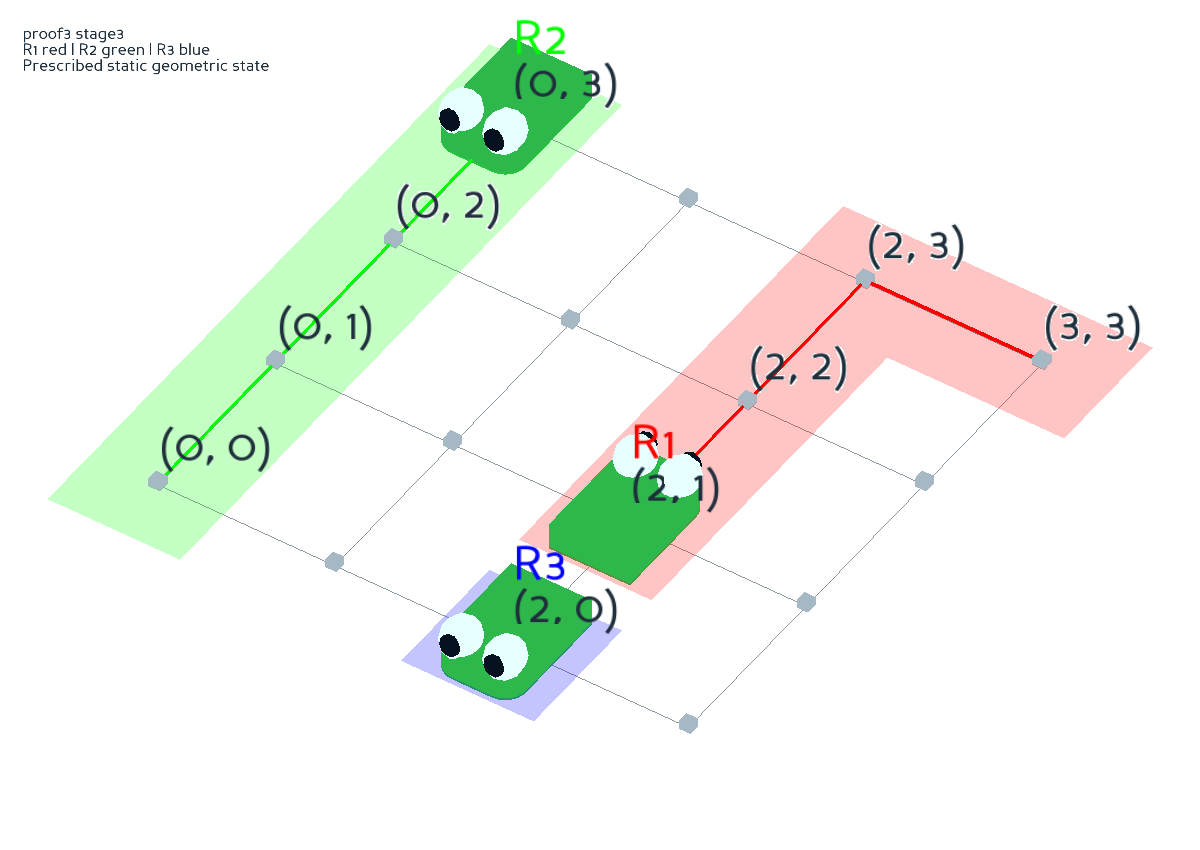
\includegraphics[height=2.65cm,keepaspectratio]{assets/proof3_stage3_white.png}\par{\scriptsize 셋째 묶음: 빨강·초록이 나머지 경로, 파랑은 대기.}
\end{column}\end{columns}

\begin{equation}
\begin{aligned}
(P_1^{(2)},P_2^{(2)})&=\bigl([(0,1),(2,1)],[(2,3),(0,3)]\bigr),\\
(P_1^{(3)},P_2^{(3)})&=\bigl([(2,1),(2,3),(3,3)],[(0,3),(0,0)]\bigr),\\
P_3^{(2)}=P_3^{(3)}&=[(2,0),(2,0)].
\end{aligned}
\tag{16}
\end{equation}
\small 둘째 묶음은 위·아래의 두 수평 경로와 파랑의 점 경로로 분리된다. 셋째 묶음도 좌측·우측의 두 경로와 파랑의 점유 영역이 서로 분리된다.
\par\smallskip\scriptsize 두 묶음 모두 식 (14)의 세 쌍을 만족한다. 수치적인 시각이나 상대 속도는 지정하지 않는다.
\end{frame}

\begin{frame}{완료 확인: 세 묶음이 정리 1의 조건을 만족한다}
\begin{columns}[T]
\begin{column}{.48\textwidth}\centering
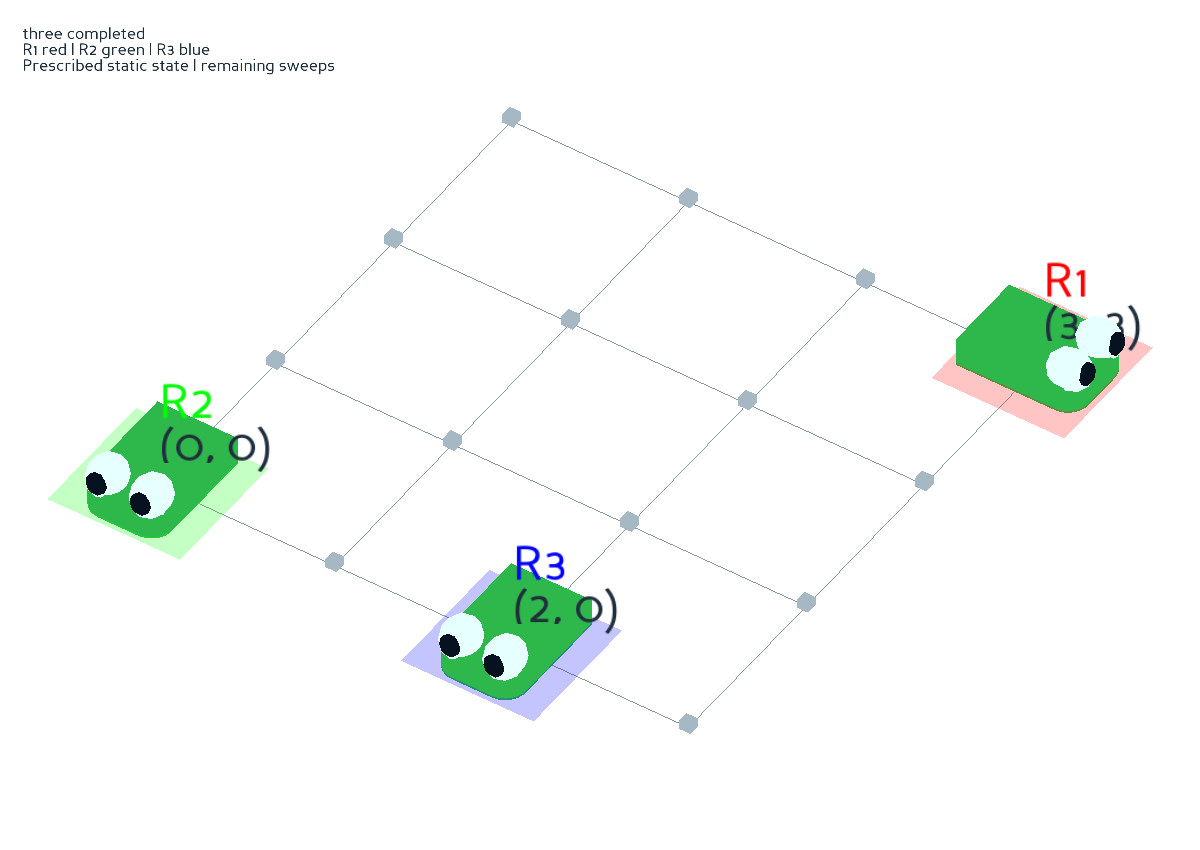
\includegraphics[height=3.35cm,keepaspectratio]{assets/three_completed_white.png}
\end{column}\begin{column}{.50\textwidth}\small
\textbf{각 묶음의 쌍별 sweep 교집합}
\begin{center}
\begin{tabular}{cccc}\toprule
묶음 & 1--2 & 1--3 & 2--3\\\midrule
1 & $\varnothing$ & $\varnothing$ & $\varnothing$\\
2 & $\varnothing$ & $\varnothing$ & $\varnothing$\\
3 & $\varnothing$ & $\varnothing$ & $\varnothing$\\\bottomrule
\end{tabular}
\end{center}
각 물체의 세 부분 경로를 연결하면 원래 경로가 된다. 대기를 포함해 공통된 세 묶음이 모두 무간섭이므로, 각 묶음을 유한시간에 실행하면 세 물체가 모두 완료한다.
\end{column}\end{columns}
\begin{equation}
\text{도착 제어점:}\quad p_1^e=(3,3),\qquad p_2^e=(0,0),\qquad p_3^e=(2,0).
\tag{17}
\end{equation}
\small 이는 \textbf{실제로 구성한 해의 증거}이다. 최적성이나 임의의 세 경로에 대한 해의 존재를 주장하지 않는다. 표는 고정된 사각형 sweep의 교집합으로 확인했다.
\end{frame}

\begin{frame}{풀리지 않는 예: 세 물체가 같은 중앙점을 지나야 한다}
\begin{columns}[T]
\begin{column}{.49\textwidth}\centering
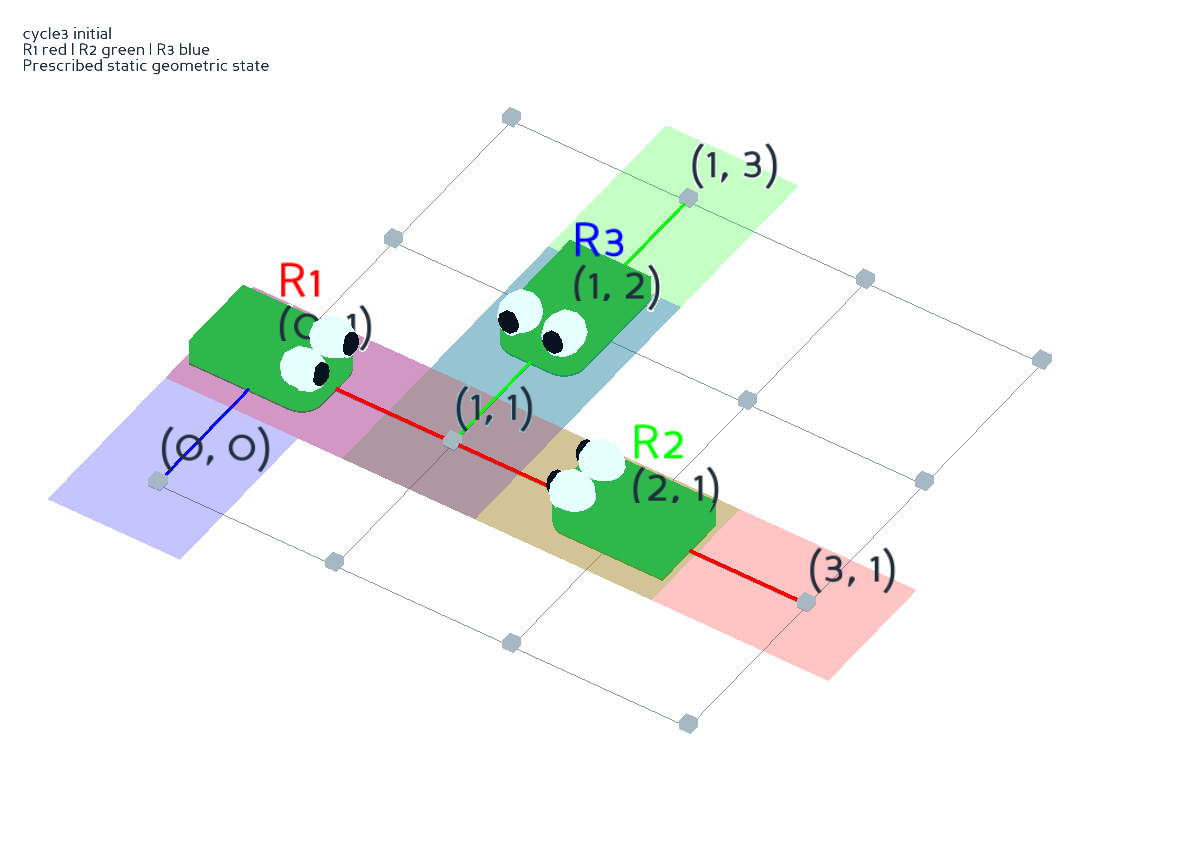
\includegraphics[height=3.65cm,keepaspectratio]{assets/cycle3_initial_white.png}
\end{column}\begin{column}{.49\textwidth}\small
\textbf{03\_06 예제}
\[
\begin{aligned}
P_1:\ &(0,1)\to(1,1)\\
&\to(2,1)\to(3,1),\\
P_2:\ &(2,1)\to(1,1)\\
&\to(1,2)\to(1,3),\\
P_3:\ &(1,2)\to(1,1)\\
&\to(0,1)\to(0,0).
\end{aligned}
\]
각 물체는 중앙 $(1,1)$을 지나, 다른 물체의 출발점을 통과해야 목적지로 갈 수 있다.
\end{column}\end{columns}
\small \textbf{이 예제의 허용 조건:} 고정 경로로 전진·대기하며, 부분 경로의 끝점은 제어점으로 제한한다. 우회·후진은 허용하지 않는다. 격자 간격은 2 m, 점유 사각형은 1.5 m이다.
\par\smallskip{\tiny\texttt{\detokenize{python -m examples.RMFS.Tests.03_06_RobotPath_ThreeWay_CyclicWait --white-background}}}
\end{frame}

\begin{frame}{왜 무간섭 묶음을 끝까지 구성할 수 없는가?}
\begin{columns}[T]
\begin{column}{.32\textwidth}\centering
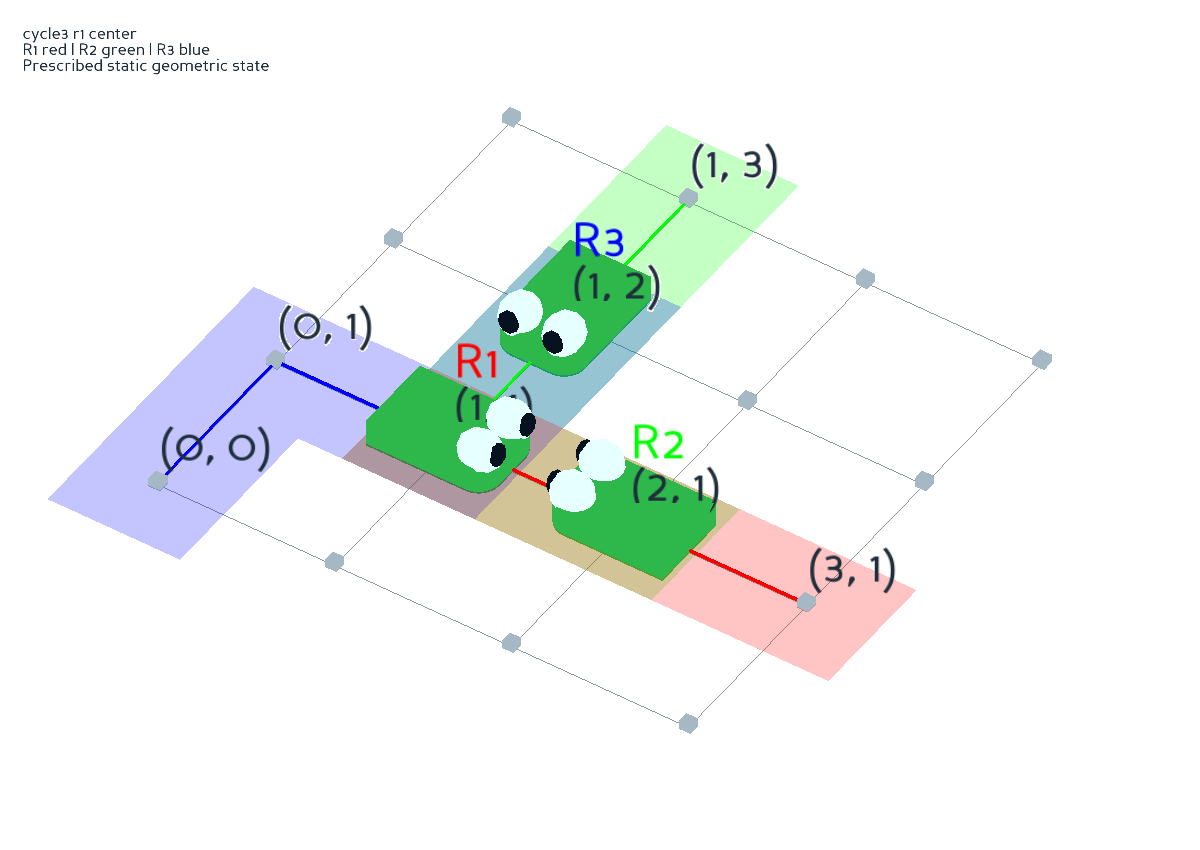
\includegraphics[height=2.1cm,keepaspectratio]{assets/cycle3_r1_center_white.png}\par{\scriptsize 빨강이 먼저 중앙에 진입.}
\end{column}\begin{column}{.32\textwidth}\centering
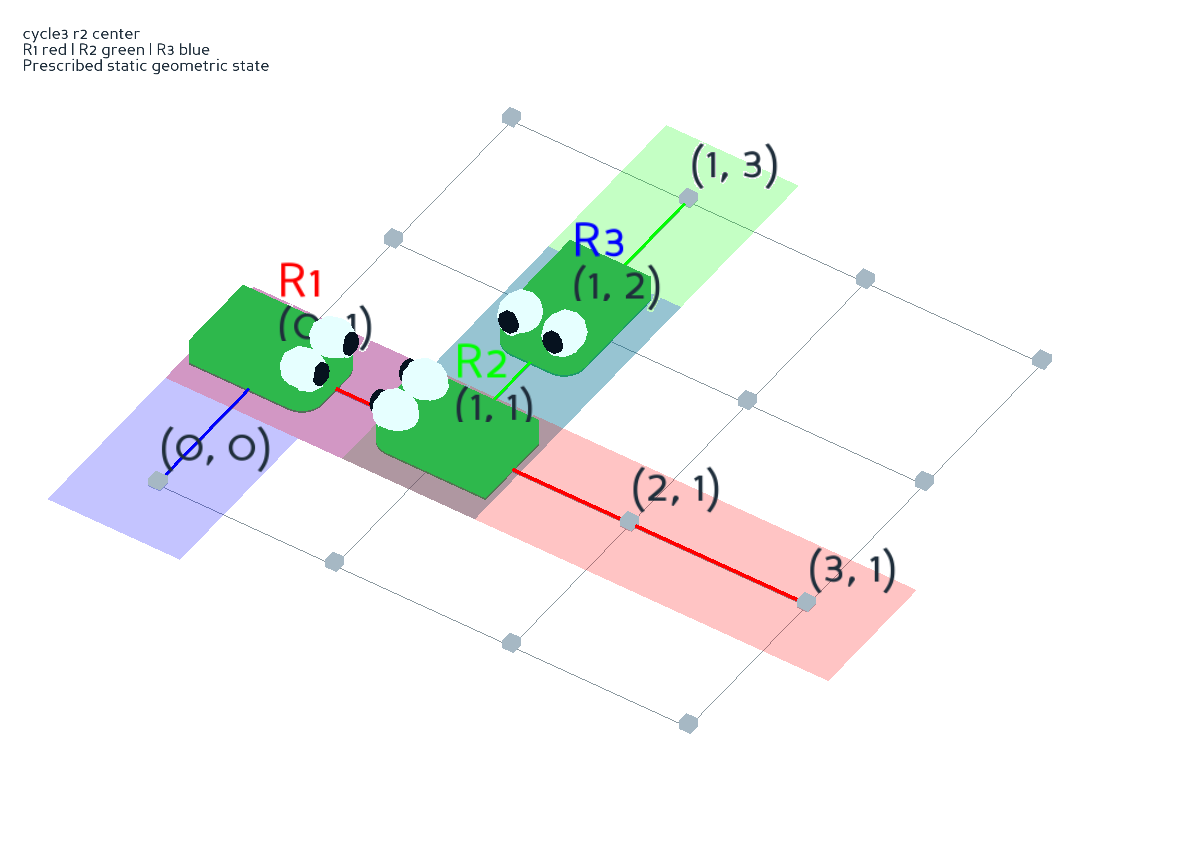
\includegraphics[height=2.1cm,keepaspectratio]{assets/cycle3_r2_center_white.png}\par{\scriptsize 초록이 먼저 중앙에 진입.}
\end{column}\begin{column}{.32\textwidth}\centering
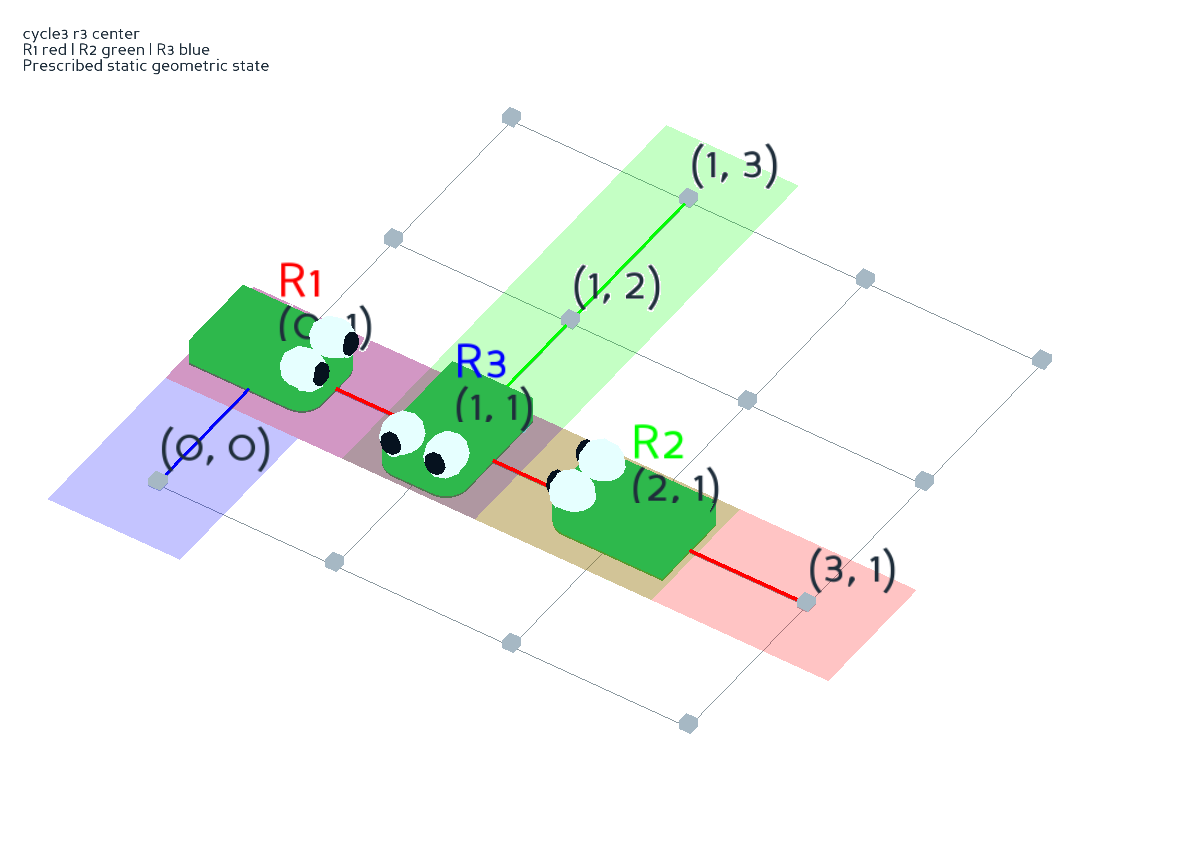
\includegraphics[height=2.1cm,keepaspectratio]{assets/cycle3_r3_center_white.png}\par{\scriptsize 파랑이 먼저 중앙에 진입.}
\end{column}\end{columns}
\small 처음으로 전진이 있는 묶음에서 두 물체 이상이 움직이면, 각 sweep이 중앙을 포함하므로 교차한다. 따라서 먼저 전진할 수 있는 것은 한 물체뿐이다.
\medskip\par
빨강이 들어간 경우, 다음 점 $(2,1)$은 초록이 점유한다. 초록과 파랑의 다음 점 $(1,1)$은 빨강이 점유한다. 다른 물체를 먼저 골라도 같은 구조로 막힌다.
\begin{equation}
(0,0,0)\longrightarrow
(1,0,0)\ \text{또는}\ (0,1,0)\ \text{또는}\ (0,0,1).
\tag{18}
\end{equation}
\scriptsize 위 숫자는 각 경로의 경유점 번호이다. 초기 0, 중앙 1, 목적지 3이다. 허용된 부분 경로 묶음을 열거하면 도달 상태는 초기와 위 세 상태뿐이며 목표 $(3,3,3)$에는 도달하지 못한다. 제자리 회전도 점유 사각형을 바꾸지 않는다.
\end{frame}








% Discussion record: audited terminology, tree structure and four operations.


\begin{frame}{확장간섭경로: 유한한 점 집합에서 경계 선택}
\small
연속인 단순 경로 $P_i:[0,1]\to Q_i$에서 상대의 전체 스윕과 간섭하는
매개변수 집합이 하나의 비어 있지 않은 구간 $[a,b]$라고 하자.
매개변수는 시간이 아니라 경로 진행 순서다.
\begin{equation}
 C_{i\mid j}=\{u:B_i(u)\cap S(P_j)\ne\varnothing\}=[a,b].\tag{24}
\end{equation}
경로 위에서 선택한 유한한 점들의 매개변수 집합을 $D_i$라 하자. 다음 두 집합이
비어 있지 않을 때 가장 가까운 앞뒤 비간섭점을 선택한다.
\begin{equation}
 a^- =\max\{d\in D_i:d<a\},\qquad
 b^+ =\min\{d\in D_i:d>b\},\qquad
 \widehat I_{i\mid j}=P_i|_{[a^-,b^+]}.\tag{25}
\end{equation}
\begin{center}\begin{tikzpicture}[x=1cm,y=1cm]
\draw[very thick,accent] (0,0)--(11,0);
\draw[line width=9pt,red!35] (4,0)--(7,0);
\draw[thick,accent,decorate,decoration={brace,amplitude=5pt}] (2,0.35)--(9,0.35)
 node[midway,above=6pt]{\footnotesize 최소 확장간섭경로};
\foreach \x/\lab in {0/0,2/{a^-},4/a,7/b,9/{b^+},11/1}
 {\fill[accent] (\x,0) circle(2pt);\node[below=5pt] at (\x,0) {$\lab$};}
\end{tikzpicture}\end{center}
\footnotesize 양 끝점의 점분스는 상대의 전체 스윕과 무간섭이다.
고정된 $D_i$에서 이 경로는 간섭경로를 포함하고 양 끝점이 비간섭점인
확장들 중 경로 포함관계상 최소이며 유일하다. 앞 또는 뒤 후보가 없으면
이 양쪽 확장은 정의되지 않는다. 이것만으로 해가 없다고 단정하지 않는다.
\end{frame}

\begin{frame}{왜 유한한 점 집합이 필요한가: 연속 경로에는 최소가 없을 수 있다}
\small
연속 경로의 모든 위치에서 정지를 허용하고 간섭 경계 $a,b$ 자체가 간섭한다면,
비간섭점 $u<a$, $v>b$를 골라도 더 가까운 점을 다시 고를 수 있다.
\begin{equation}
 u<\frac{u+a}{2}<a,\qquad
 b<\frac{b+v}{2}<v.\tag{26}
\end{equation}
따라서 양 끝점이 비간섭인 확장경로는 존재해도,
\textbf{가장 짧은 확장경로는 존재하지 않을 수 있다.}
간섭 경계까지 접근하는 극한을 실제 비간섭 정지점으로 사용할 수는 없다.
\begin{center}\begin{tikzpicture}[x=1cm,y=1cm]
\draw[thick,accent] (0,0)--(11,0);
\draw[line width=8pt,red!35] (6,0)--(10,0);
\foreach \x in {1,3.5,4.75,5.375,5.6875}
 {\fill[accent] (\x,0) circle(2pt);}
\fill[red!70!black] (6,0) circle(3pt);
\node[below] at (6,-.1) {$a$: 간섭 경계};
\draw[->,accent,thick] (1,.5)--(5.7,.5)
 node[midway,above]{\footnotesize 더 가까운 비간섭점을 계속 선택 가능};
\end{tikzpicture}\end{center}
\textbf{유한한 점 집합은 선택 가능한 경계를 이산화한다.}
앞뒤 후보가 존재하면 유한 집합의 최댓값과 최솟값으로 최소 확장이 정해진다.
\par\medskip\footnotesize
이는 경로 위에 유한한 점 집합을 지정하는 수학적 이유다. 다만 실제 정지 가능 여부와 안전 여유는
별도 조건이다. 여기서는 기하학적 비간섭을 다루며, 전체 완료의 필요충분조건은
아직 증명하지 않았다.
\end{frame}

\begin{frame}{짝 경로의 구성 문제: 시작경로와 끝경로}
\small
여기서는 스윕을 잠시 제외하고 두 연속 단순 경로 $P_i:[0,1]\to Q$,
$i=1,2$의 경로 영역을 다룬다. 상대 경로와 교차하는 부분의 매개변수 집합을
\begin{equation}
 C_i=\{u\in[0,1]:P_i(u)\in\operatorname{im}P_j\},\qquad j\ne i
 \tag{27}
\end{equation}
로 정의한다. $\operatorname{im}P_j$는 상대 경로의 전체 영역이다.
비어 있지 않은 $C_i$의 첫 경계와 마지막 경계를 $a_i=\min C_i$,
$b_i=\max C_i$라 하면,
\begin{equation}
 P_i^-=P_i|_{[0,a_i)},\qquad P_i^+=P_i|_{(b_i,1]}
 \tag{28}
\end{equation}
를 각각 \textbf{시작경로}, \textbf{종경로(끝경로)}라 한다.
간섭 부분이 여러 개여도 전체 간섭집합의 첫 경계와 마지막 경계를 사용한다.
\begin{center}\begin{tikzpicture}[x=1cm,y=1cm]
\draw[line width=4pt,accent] (0,0)--(3,0);
\draw[line width=4pt,red!45] (3,0)--(5,0);
\draw[line width=4pt,accent] (5,0)--(7,0);
\draw[line width=4pt,red!45] (7,0)--(8,0);
\draw[line width=4pt,accent] (8,0)--(11,0);
\node[below] at (1.5,0){\footnotesize 시작경로};
\node[below] at (5.5,0){\footnotesize 간섭·비간섭 부분};
\node[below] at (9.5,0){\footnotesize 끝경로};
\node[above] at (0,0){$s_i$};\node[above] at (3,0){$a_i$};
\node[above] at (8,0){$b_i$};\node[above] at (11,0){$e_i$};
\end{tikzpicture}\end{center}
\footnotesize 간섭이 전혀 없으면 두 전체 경로 자체가 무간섭이다.
그림의 구간 길이는 개념도이며 수치적인 시간을 뜻하지 않는다.
\end{frame}

\begin{frame}{분스복과 분스합}
\small
\textbf{분스}는 부분 경로의 스윕이며, \textbf{점분스}는 한 점경로에서의 점유 영역이다.
경로를 구성하는 분스의 순서는 유지한다.
\begin{center}\begin{tikzpicture}[x=1cm,y=1cm]
\node[left] at (0,1.4){\textbf{분스복}};
\node[draw,minimum width=.8cm] at (1,1.4){$p$};
\draw[->,thick,accent] (2,1.4)--(3,1.4);
\foreach \x in {4,5,6}{\node[draw,minimum width=.8cm] at (\x,1.4){$p$};}
\node[right] at (7,1.4){\footnotesize 같은 점에서 대기};
\node[left] at (0,0){\textbf{분스합}};
\node at (1,0){$e_{ab}$};\node at (2,0){$p_b$};\node at (3,0){$e_{bc}$};
\draw[->,thick,accent] (3.7,0)--(4.7,0);
\node[draw,minimum width=1.3cm] at (5.8,0){$e_{ac}$};
\node[right] at (7,0){\footnotesize 중간점을 통과};
\end{tikzpicture}\end{center}
\textbf{분스복:} 점분스를 같은 위치에 복사·삽입하여 대기를 추가한다.
다른 물체의 이동 부분과 짝을 맞추는 데 사용하며, 복사 횟수는 대기시간이 아니다.
\par\medskip
\textbf{분스합:} 연속된 이동과 중간 점분스를 하나의 이동 분스로 묶는다.
원래 경유 경로를 유지하며, 중간점의 별도 정지를 없앤다.
합친 후에도 상대와의 무간섭성과 실제 운동 가능성을 확인해야 한다.
\par\medskip
\textbf{현재 목적:} 분스복으로 충돌 없는 짝 경로의 존재를 증명한다.
분스합을 통한 효율화는 이후에 다룬다.
\end{frame}

\begin{frame}{정리 2: 분스복으로 무간섭 짝 경로를 구성하는 충분조건}
\small
\textbf{가정.} 두 원 경로는 유한한 점경로·이동 부분경로의 순서열로 주어지고,
각 이동은 실행 가능하다. 점경로에서는 대기할 수 있다.
각 원 경로에서 간섭경로를 제외한 양쪽에 비어 있지 않은 시작경로와 끝경로가 남는다.
\par\medskip
\textbf{주장.} 원 경로의 이동 순서를 보존하면서, \textbf{점경로의 복사 연산(대기)}으로
두 원 경로를 모두 완주하는 무간섭 짝 경로를 구성할 수 있다.
\par\medskip
$P_1$의 구성 순서열을 $A_1,\ldots,A_r$, $P_2$를 $B_1,\ldots,B_s$라 하자.
$\langle s_1\rangle$은 물체 1의 시작 점경로,
$\langle e_2\rangle$는 물체 2의 종점경로다. 다음과 같이 짝짓는다.
\begin{equation}
 \mathcal P=\bigl(
 (\langle s_1\rangle,B_1),\ldots,(\langle s_1\rangle,B_s),
 (A_1,\langle e_2\rangle),\ldots,(A_r,\langle e_2\rangle)
 \bigr).
 \tag{29}
\end{equation}
\begin{center}\begin{tikzpicture}[x=1cm,y=1cm]
\node[left] at (0,.65){\footnotesize 물체 1};
\node[left] at (0,-.2){\footnotesize 물체 2};
\draw[thick,accent] (0,.65)--(5,.65);
\node[above] at (2.5,.65){\footnotesize 시작 점경로 복사: 대기};
\draw[->,very thick,red!65!black] (5,.65)--(11,.65);
\node[above] at (8,.65){\footnotesize $A_1,\ldots,A_r$ 이동};
\draw[->,very thick,red!65!black] (0,-.2)--(5,-.2);
\node[below] at (2.5,-.2){\footnotesize $B_1,\ldots,B_s$ 이동};
\draw[thick,accent] (5,-.2)--(11,-.2);
\node[below] at (8,-.2){\footnotesize 종점경로 복사: 대기};
\draw[dashed] (5,-.6)--(5,1.15);
\end{tikzpicture}\end{center}
\footnotesize 시작점과 종점은 원 순서열에 이미 존재한다. 복사본만 삽입하며,
원래의 구성 항목을 삭제하거나 순서를 바꾸지 않는다. 도식의 가로축은 실행 순서다.
\end{frame}

\begin{frame}{정리 2의 증명과 후속 과제}
\small
\textbf{증명.} 시작경로가 비어 있지 않으므로 $s_1$은 상대의 전체 경로 영역 밖에 있다.
따라서 물체 1이 $s_1$에서 대기하는 동안 물체 2의 모든 구성 항목 $B_k$와 무간섭이다.
\par\medskip
마찬가지로 끝경로가 비어 있지 않으므로 $e_2$는 물체 1의 전체 경로 영역 밖에 있다.
물체 2가 $e_2$에서 대기하는 동안 물체 1의 모든 구성 항목 $A_k$와 무간섭이다.
따라서 식 (29)의 모든 짝은 무간섭이다.
\par\medskip
각 물체의 성분을 순서대로 연결하면, 원 경로에 점경로의 반복만 추가된다.
그러므로 원래 이동 순서를 유지하며 두 원 경로를 완주한다.
짝의 개수는 유한하며, 각 짝이 유한시간에 실행되면 전체 실행도 유한시간에 끝난다.
\hfill$\square$
\par\medskip
\textbf{정리의 범위.} 해의 존재를 보이는 \textbf{충분조건}이다.
필요조건이나 최소 makespan을 주장하지 않는다. 증명은 전체 간섭집합을 사용하므로
간섭 부분이 여러 개여도 동일하게 적용되며, 구간별 우선순위를 따로 정할 필요가 없다.
\par\medskip
\textbf{후속 과제.} 지금은 분스복으로 안전한 짝 경로의 존재를 확보한다.
부분경로의 합(분스합)을 이용해 정지·대기를 줄이는 효율화는 이후에 다룬다.
\par\smallskip\footnotesize
실제 크기가 있는 이동물체로 적용할 때는 식 (27)의 경로 교차를 점유 영역과
스윕의 간섭 판정으로 바꾸고 같은 증명 구조를 적용한다.
\end{frame}

\begin{frame}{단위 경로쌍과 필요성 증명에 사용하는 공통 부분경로}
\small
\textbf{단위 경로쌍}은 간섭경로가 하나 이하인 두 경로의 쌍이다.
스윕 교집합이 비어 있으면 \textbf{상호 독립 경로}라 한다.
이 정의에 격자 크기나 간격은 포함하지 않는다.
\par\medskip
정리 4의 필요성을 증명할 때에는 두 중심 경로의 공통 부분을 별도로 사용한다.
\begin{equation}
 K_{ij}=\operatorname{im}P_i\cap\operatorname{im}P_j.
 \tag{35}
\end{equation}
그 증명은 $K_{ij}$가 비어 있거나 \textbf{하나의 연결된 공통 부분경로}라는
추가 가정을 사용한다. 한 점에서만 만나는 경우도 포함한다.
\begin{center}\begin{tikzpicture}[x=1cm,y=1cm]
\draw[very thick,red!65] (0,0)--(8,0);
\draw[very thick,blue!65] (2,1)--(2,0)--(6,0)--(6,1);
\draw[line width=5pt,purple!60] (2,0)--(6,0);
\node[below] at (4,0){$K_{ij}$: 하나의 공통 부분경로};
\end{tikzpicture}\end{center}
\textbf{사용처:} 공통 부분의 진행 순서를 뒤집으려면 서로 만나야 한다는 논리와,
양 끝이 공통 부분에 있으면 그 사이 경로도 그 부분에 포함된다는 논리에 사용한다.
정리 2·3의 충분성 구성에는 이 추가 가정이 필요하지 않다.
\par\medskip
\textbf{구별:} $K_{ij}$는 중심 경로의 공통 부분이고,
$S_i(P_i)\cap S_j(P_j)$는 공간상의 스윕 교집합이다.
또 식 (24)의 $C_{i\mid j}$는 자기 경로의 \textbf{진행 매개변수 집합}이다.
세 집합을 같은 것으로 쓰지 않는다.
\end{frame}

\begin{frame}{네 끝점의 간섭과 세 불가능 유형}
\small
시작점 $s_i$, 종점 $e_i$는 기존 기호를 유지한다.
진위 표시는 좌표와 혼동하지 않도록 $\sigma_i,\varepsilon_i$를 쓴다.
\begin{equation}
 \sigma_i=\mathbf1\{B_i(0)\cap S_j(P_j)\ne\varnothing\},\qquad
 \varepsilon_i=\mathbf1\{B_i(1)\cap S_j(P_j)\ne\varnothing\}.
 \tag{36}
\end{equation}
\begin{equation}
 H_s=\sigma_i\land\sigma_j,\quad
 H_e=\varepsilon_i\land\varepsilon_j,\quad
 H_b=(\sigma_i\land\varepsilon_i)\lor(\sigma_j\land\varepsilon_j).
 \tag{37}
\end{equation}
\begin{center}\begin{tikzpicture}[x=.75cm,y=.65cm]
\foreach \y/\lab in {2/{종착 간섭쌍 $H_e$},0/{시작 간섭쌍 $H_s$},-2/{막힘 간섭쌍 $H_b$}} {
\fill[red!45] (0,\y) rectangle (3,\y+.6);
\fill[blue!45] (3,\y) rectangle (4.5,\y+.6);
\fill[purple!50] (2,\y) rectangle (3,\y+.6);
\node[right] at (5,\y+.3){\lab};}
\draw[->,thick] (.3,2.3)--(1.5,2.3);\draw[->,thick] (4.2,2.3)--(3.3,2.3);
\draw[->,thick] (1.5,.3)--(.3,.3);\draw[->,thick] (3.3,.3)--(4.2,.3);
\fill[red!45] (3,-2) rectangle (4.5,-1.4);
\fill[purple!50] (1.5,-2) rectangle (3,-1.4);
\draw[<->,thick] (.2,-1.7)--(4.3,-1.7);
\draw[<->,thick,blue!70!black] (1.7,-1.7)--(2.8,-1.7);
\end{tikzpicture}\end{center}
\footnotesize 세 유형은 서로 배타적이지 않다. $H_b$는 한 물체의 양 끝 간섭이라는
검사식이다. 이것이 막힘을 뜻한다는 주장은 앞 페이지의 공통 통로 범위에서 사용한다.
일반 스윕의 포함관계만으로 해 없음을 주장하지 않는다.
\end{frame}

\begin{frame}{16가지 끝점 유형: 공통 통로 범위의 분류}
\footnotesize\renewcommand{\arraystretch}{1.02}
\begin{center}\begin{tabular}{rcccccl}\toprule
번호 & $\sigma_i$ & $\varepsilon_i$ & $\sigma_j$ & $\varepsilon_j$ & $F_{ij}$ & 직렬 통과 구성 또는 불가 유형\\\midrule
1 & 0&0&0&0 & 1 & 어느 쪽이든 선행\\
2 & 0&0&0&1 & 1 & $i$ 선행\\
3 & 0&0&1&0 & 1 & $j$ 선행\\
4 & 0&0&1&1 & 0 & $H_b$\\
5 & 0&1&0&0 & 1 & $j$ 선행\\
6 & 0&1&0&1 & 0 & $H_e$\\
7 & 0&1&1&0 & 1 & $j$ 선행\\
8 & 0&1&1&1 & 0 & $H_e,H_b$\\
9 & 1&0&0&0 & 1 & $i$ 선행\\
10 & 1&0&0&1 & 1 & $i$ 선행\\
11 & 1&0&1&0 & 0 & $H_s$\\
12 & 1&0&1&1 & 0 & $H_s,H_b$\\
13 & 1&1&0&0 & 0 & $H_b$\\
14 & 1&1&0&1 & 0 & $H_e,H_b$\\
15 & 1&1&1&0 & 0 & $H_s,H_b$\\
16 & 1&1&1&1 & 0 & $H_s,H_e,H_b$\\\bottomrule
\end{tabular}\end{center}
\begin{equation}
 F_{ij}=(\neg\sigma_j\land\neg\varepsilon_i)
 \lor(\neg\sigma_i\land\neg\varepsilon_j)
 =\neg(H_s\lor H_e\lor H_b).
 \tag{38}
\end{equation}
\scriptsize $F_{ij}$는 완결 가능성(Feasibility)이며 1은 해 있음, 0은 해 없음이다.\par 선행은 간섭구간을 한 대씩 처리하는 구성 순서다.
세 불가 유형의 합집합은 9가지, 그 밖의 완결 가능 유형은 7가지다.
\end{frame}

\begin{frame}{정리 4: 하나의 공통 통로에 대한 분류와 증명}
\small
\textbf{추가 가정.} $K_{ij}$는 비어 있거나 하나의 공통 부분경로다.
각 시작·종점에서는 \textbf{점분스와 상대 스윕의 간섭 여부가,
그 점이 상대 중심 경로 위에 놓이는지와 일치}한다고 하자.
경로의 진행 순서는 고정하며 대기는 허용한다.
\par\smallskip
\textbf{정리 4.} 이 가정 아래,
진행과 점경로 복사로 두 경로를 완결할 수 있는 것과 $F_{ij}=1$은 동치다.
\par\smallskip
\textbf{충분성.} $\sigma_j=0,\varepsilon_i=0$이면 $j$는 안전한 시작점에서 대기하고
$i$가 원 경로를 완료한다. 이어 $i$는 안전한 종점에서 대기하고 $j$가 완료한다.
반대 항도 역할을 바꾸어 같은 구성으로 증명된다.
원 구성열 사이에 점경로만 복사하므로 분스합은 필요 없다.
\par\smallskip
\textbf{필요성.} $F_{ij}=0$이면 다음 중 하나가 성립한다.
\begin{itemize}
\item $H_s$: 두 시작점이 공통 통로에 있다. 시작점이 같으면 초기 충돌이다.
다르면 두 단순 경로가 공통 통로를 반대 순서로 따라야 하므로 서로 지나쳐야 한다.
\item $H_e$: 두 종점이 공통 통로에 있다. 같은 종점이면 완료 시 충돌이다.
다르면 공통 통로에서 서로 지나쳐야 한다.
\item $H_b$: 한 물체의 경로 양 끝이 공통 부분경로에 있다.
공통 부분이 연결되어 있으므로 그 물체의 경로 전체가 상대 경로의 부분경로다.
상대가 이를 처음부터 끝까지 통과하려면 안의 물체를 지나쳐야 한다.
\end{itemize}
공통 통로 위의 연속적인 진행에서 두 중심의 순서를 바꾸려면 같은 점에서 만나야 한다.
대기는 이 순서 역전의 불가능성을 바꾸지 않는다. 따라서 해가 없다.\hfill$\square$
\par\smallskip\scriptsize 일반 스윕에 대한 확대에는 별도의 증명이 필요하다.
\end{frame}

\begin{frame}{표에서 얻는 관계: 직렬 통과 구성의 선행 요구}
\small
간섭구간을 한 대씩 처리하는 구성에서, $i\mathrel{\mathop{\to}\limits^{\rm ser}_{ij}}j$를
「$i$보다 $j$를 먼저 통과시켜야 한다」는 요구로 정의한다.
\begin{equation}
 i\mathrel{\mathop{\to}\limits^{\rm ser}_{ij}}j
 \iff\sigma_j\lor\varepsilon_i,\qquad
 j\mathrel{\mathop{\to}\limits^{\rm ser}_{ij}}i
 \iff\sigma_i\lor\varepsilon_j.
 \tag{39}
\end{equation}
\begin{center}\begin{tikzpicture}
\node[module] (i) at (-3,0){물체 $i$};
\node[module] (j) at (3,0){물체 $j$};
\draw[flow] (i) to[bend left=15] node[lab,above]{$\sigma_j\lor\varepsilon_i$}(j);
\draw[flow] (j) to[bend left=15] node[lab,below]{$\sigma_i\lor\varepsilon_j$}(i);
\end{tikzpicture}\end{center}
화살표 없음: 1유형, 단방향: 각 3유형, 양방향: 불가한 9유형이다.
\par\medskip
\textbf{의미 제한:} 이 관계는 직렬 통과 구성을 위한 요구다.
모든 안전 실행에서 상대가 간섭구간 전체를 이탈할 때까지 기다려야 한다는 뜻이 아니다.
같은 방향에서는 앞 물체가 필요한 부분을 비우면 뒤 물체가 뒤따를 수 있다.
전체 경로의 완주 순서나 현재 시점의 실제 대기 상태와도 동일시하지 않는다.
\end{frame}

\begin{frame}{현재 대기 관계: 상태와 요청 부분경로}
\small
현재 진행 상태를 $q=(u_1,\ldots,u_n)$, 물체 $i$가 요청한 다음 부분경로를 $A_i$라 하자.
현재 점유가 그 이동을 막는 관계는 다음처럼 별도로 표현할 수 있다.
\begin{equation}
 i\mathrel{\mathop{\to}\limits^{q,A}}j
 \iff i\ne j\ \land\ S_i(A_i)\cap B_j(u_j)\ne\varnothing.
 \tag{40}
\end{equation}
이는 $j$를 현재 위치에 세워 두면 $i$가 요청한 이동 전체를 실행할 수 없다는 뜻이다.
$j$가 실제로 비킬 수 있는지, 어느 부분까지 해제해야 하는지는 추가로 확인한다.
\par\medskip
\begin{center}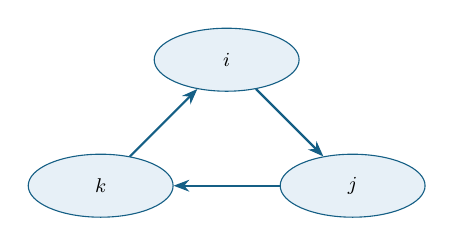
\begin{tikzpicture}[scale=.8,transform shape]
\foreach \name/\lab/\x/\y in {a/i/0/1.3,b/j/2/-.7,c/k/-2/-.7}
 {\node[phase] (\name) at (\x,\y){$\lab$};}
\draw[flow] (a)--(b);\draw[flow] (b)--(c);\draw[flow] (c)--(a);
\end{tikzpicture}\end{center}
\textbf{복수 물체:} 모든 쌍이 완결 가능해도 의존관계가 순환할 수 있다.
다만 이동 단위를 더 짧게 바꾸거나 다른 안전한 진행이 있으면 순환을 해소할 수도 있다.
따라서 단순한 경로 교차나 선택한 우선순위의 순환만으로 교착을 확정하지 않는다.
\par\smallskip\footnotesize
위 관계는 정의 제안이며 아직 TrafficManager의 구현 규칙으로 교체하지 않았다.
물체가 이미 종점에 있어 비킬 수 없는 막힘은 순환 없이도 발생할 수 있다.
\end{frame}

\begin{frame}{실험 기록: 16개 유형, 1,799,096개 경로쌍}
\small
4$\times$4 격자에서 1--5선분의 단순 경로 1,616개를 생성하고 모든 순서 있는 경로쌍을 열거했다.
격자 간격은 2 m, 물체는 축 정렬된 1.5 m 정사각형이다.
이 예에서는 정리 4의 끝점 간섭과 중심 경로 포함의 판정이 일치한다.
동일한 시작 위치는 제외하고, 공통 중심 경로가 비어 있거나 하나로 연결된 쌍을 검사했다.
\begin{center}\begin{tabular}{lrr}\toprule
분류 & 끝점 유형 수 & 검사한 경로쌍 수\\\midrule
완결 가능 & 7 & 1,586,016\\
완결 불가능 & 9 & 213,080\\\midrule
합계 & 16 & 1,799,096\\\bottomrule
\end{tabular}\end{center}
정수 좌표로 계산하는 독립적인 정점 진행 DAG와 식 (38)의 판정이 모두 일치했다.
각 유형 20개씩 총 320개는 실제 WaitDuplicationSolver로도 교차 검사했고,
성공한 묶음 경로의 무간섭과 전체 완료를 재검사했다.
\par\medskip
\textbf{검사하지 않은 범위:} 6선분 이상의 경로, 다른 격자·물체 크기,
회전하는 점유 형상, 일반적인 곡선 스윕 및 복수 물체 전체의 필요충분성.
실험은 명시한 범위의 증거이며 일반화를 대신하지 않는다.
\par\smallskip\scriptsize
실행: \texttt{\detokenize{python -m examples.RMFS.Tests.run_unit_pair_classification --max-edges 5}}\par
결과: \texttt{Tests/results/unit\_pair\_classification.json}.
검증기 외에 기존 Plant·TrafficManager 실행 규칙은 이 실험 때문에 변경하지 않았다.
\end{frame}

\begin{frame}{간섭 진행 구간 하나와 공통 통로 하나는 다르다}
\begin{columns}[T]
\begin{column}{.43\textwidth}\centering
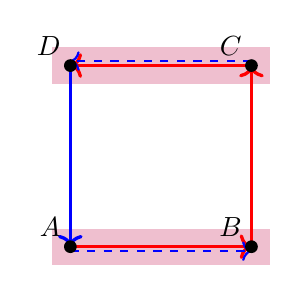
\begin{tikzpicture}[scale=1.15]
\fill[purple!25] (-.2,-.2) rectangle (2.2,.2);
\fill[purple!25] (-.2,1.8) rectangle (2.2,2.2);
\draw[->,very thick,red] (0,0)--(2,0);
\draw[->,very thick,red] (2,0)--(2,2);
\draw[->,very thick,red] (2,2)--(0,2);
\draw[->,blue,thick,dashed] (2,2.05)--(0,2.05);
\draw[->,blue,very thick] (0,2)--(0,0);
\draw[->,blue,thick,dashed] (0,-.05)--(2,-.05);
\foreach \x/\y/\lab in {0/0/A,2/0/B,2/2/C,0/2/D}
 {\fill (\x,\y) circle(2pt);\node[above left] at (\x,\y){$\lab$};}
\end{tikzpicture}
\end{column}\begin{column}{.55\textwidth}\small
2 m 간격 정사각형의 꼭짓점 순서를 $A,B,C,D$라 하자.
\[
 P_i:A\to B\to C\to D,\qquad
 P_j:C\to D\to A\to B.
\]
두 물체가 반대편 변들을 동시에 이동하면 세 묶음으로 완료한다.
초기 $A,C$와 종점 $D,B$는 모두 상대 경로 위에 있다.
\par\medskip
하지만 공통 중심 경로는 $AB$와 $CD$ \textbf{두 조각}이다.
따라서 식 (35)의 단일 공통 통로 분류 대상이 아니다.
\end{column}\end{columns}
\par\medskip\small
반면 현재 물체 크기에서는 각 물체의 간섭 진행 집합 $C_{i\mid j}$가 경로 전체로 이어질 수 있다.
이를 기준으로만 단위를 정의하면 위 예가 1111 유형이면서 풀리는 반례가 된다.
\textbf{따라서 단위의 연결성이 어느 집합에 대한 것인지 반드시 명시해야 한다.}
\end{frame}


\begin{frame}{정리 3 개정: 쌍별 선행 요구를 복수 물체로 확장}
\small
앞의 쌍별 분류 뒤에서 정리 3을 다시 서술한다. 원래 정리 3의 번호는 유지한다.
물체 $i$의 시작·종점과 상대 $j$의 전체 스윕으로 계산하는 진위를
$\sigma_{i\mid j},\varepsilon_{i\mid j}$라 쓰자. 식 (36)의 상대를 명시한 것이다.
\par\medskip
직렬 통과 구성을 위한 선행 요구를 모든 물체 쌍에 대해 모은다.
\begin{equation}
 D=(\{1,\ldots,n\},E),\qquad
 (i,j)\in E\iff\sigma_{j\mid i}\lor\varepsilon_{i\mid j}.
 \tag{41}
\end{equation}
화살표 $i\to j$는 이 구성에서 $j$를 먼저 처리하라는 뜻이다.
따라서 실행 순서는 화살표의 반대 방향으로 정렬한다.
\begin{center}\begin{tikzpicture}
\node[phase] (a) at (-3,0){$1$};\node[phase] (b) at (0,0){$2$};
\node[phase] (c) at (3,0){$3$};
\draw[flow] (a)--(b);\draw[flow] (b)--(c);
\node at (0,-1){실행 순서: $3,2,1$};
\end{tikzpicture}\end{center}
\footnotesize 각 쌍이 정리 4의 범위에 있으면, 세 불가 유형은 양방향 요구로 나타난다.
아래 충분성 증명은 끝점 점유와 전체 스윕의 관계만 사용하므로,
각 쌍의 간섭구간이 하나라는 가정 없이도 적용된다.
\end{frame}

\begin{frame}{정리 3 개정: 비순환 선행 요구는 완결의 충분조건}
\small
\textbf{정리 3.} 유한한 물체들의 원 경로가 실행 가능한 유한한 구성열로 주어지고
점경로에서 대기할 수 있다고 하자. 식 (41)의 그래프 $D$가 비순환이면,
분스복으로 모든 원 경로를 완주하는 무간섭 묶음 경로를 구성할 수 있다.
\par\medskip
비순환성이 보장하는 실행 순위를 $\rho$로 정한다.
\begin{equation}
 (i,j)\in E\ \Longrightarrow\ \rho(j)<\rho(i).
 \tag{42}
\end{equation}
순위가 낮은 물체부터 한 대씩 완주시킨다.
아직 출발하지 않은 물체는 시작점, 이미 완료한 물체는 종점에서 점경로를 복사해 대기한다.
\par\medskip
\textbf{증명: 움직이는 물체와 대기 물체.}
물체 $i$의 차례에서, 뒤에 실행할 $j$는 시작점에 있다.
만약 $\sigma_{j\mid i}=1$이면 $i\to j$여서 $j$가 먼저 실행돼야 한다.
이는 순서에 모순이므로 $j$의 시작점은 $i$의 전체 스윕과 무간섭이다.
\par\medskip
이미 완료한 $j$는 종점에 있다. 만약 $\varepsilon_{j\mid i}=1$이면 $j\to i$여서
$i$가 먼저 실행돼야 한다. 역시 모순이므로 $j$의 종점은 $i$의 전체 스윕과 무간섭이다.
따라서 움직이는 $i$는 모든 대기 물체와 무간섭이다.
\end{frame}

\begin{frame}{정리 3의 증명 계속: 대기 물체들과 전체 완료}
\small
\textbf{대기 물체끼리의 무간섭.}
아직 시작하지 않은 두 물체의 시작점유가 겹치면 두 시작 진위가 모두 1이므로
양방향 화살표가 생긴다. 이미 완료한 두 물체의 종점유가 겹치는 경우도 같다.
이는 $D$의 비순환성에 모순이다.
\par\medskip
이미 완료한 물체 $j$의 종점유와 아직 출발하지 않은 물체 $k$의 시작점유가 겹친다고 하자.
$k$의 시작점유는 자기 전체 스윕에 포함되므로 $\varepsilon_{j\mid k}=1$이다.
따라서 $j\to k$로 $k$가 먼저 실행돼야 하지만, 현재는 $j$가 먼저 완료했으므로 모순이다.
대기 물체들 사이에도 충돌이 없다.
\par\medskip
각 단계에서 한 물체가 안전하게 완주하고 나머지는 안전하게 대기한다.
유한한 물체 수에 대해 반복하면 모두 완료한다.
원 구성 항목은 원래 순서대로 실행하며 추가 항목은 점경로의 복사뿐이다.
각 구성 항목의 실행시간이 유한하면 전체 실행시간도 유한하다.\hfill$\square$
\par\medskip
\textbf{기존 결과와의 관계.} 이전 정리 3의 모든 시작·종점 비간섭 조건이면
$E=\varnothing$이므로 이 개정 정리의 특별한 경우다.
시작·종점 간섭이 있어도 요구가 비순환이면 이제 허용된다.
\par\smallskip\footnotesize
필요충분조건이나 최소 makespan 정리가 아니다.
쌍별 완결 가능성만으로 전체 완결 가능성을 결론 내리지 않는다.
\end{frame}

\begin{frame}{순환이 있어도 풀리는 예: 정적 선행 요구와 실제 대기의 차이}
\begin{columns}[T]
\begin{column}{.43\textwidth}\centering
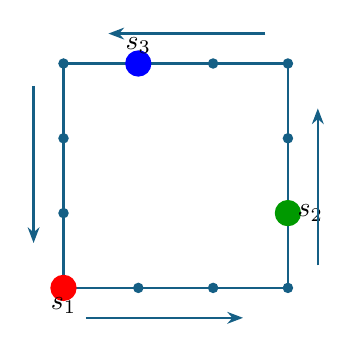
\begin{tikzpicture}[scale=.95]
\draw[accent,thick] (0,0) rectangle (3,3);
\foreach \x/\y in {0/0,1/0,2/0,3/0,3/1,3/2,3/3,2/3,1/3,0/3,0/2,0/1}
 {\fill[accent] (\x,\y) circle(2pt);}
\fill[red] (0,0) circle(5pt);\node[below] at (0,0){$s_1$};
\fill[green!60!black] (3,1) circle(5pt);\node[right] at (3,1){$s_2$};
\fill[blue] (1,3) circle(5pt);\node[above] at (1,3){$s_3$};
\draw[flow] (.3,-.4)--(2.4,-.4);
\draw[flow] (3.4,.3)--(3.4,2.4);
\draw[flow] (2.7,3.4)--(.6,3.4);
\draw[flow] (-.4,2.7)--(-.4,.6);
\end{tikzpicture}
\end{column}\begin{column}{.55\textwidth}\small
4$\times$4 격자의 바깥 둘레를 같은 방향으로 이동하는 세 물체다.
\[
\begin{aligned}
P_1:&\ (0,0)\to(3,0)\to(3,2),\\
P_2:&\ (3,1)\to(3,3)\to(0,3),\\
P_3:&\ (1,3)\to(0,3)\to(0,0)\to(1,0).
\end{aligned}
\]
각 경로는 인접 정점 다섯 선분으로 펼친다.
각 쌍은 단위 공통 통로이며 모두 완결 가능하지만,
식 (41)에는 $1\to2\to3\to1$이 생긴다.
\end{column}\end{columns}
\par\medskip\small
세 물체가 간격을 유지하며 함께 전진하면 완료할 수 있다.
실제 분스복 Solver에서도 11개 묶음의 해를 찾아 무간섭·완주를 재검사했다.
따라서 \textbf{정적 그래프 $D$의 순환만으로 전체 불가능을 판정할 수 없다.}
반면 03\_06 예제는 실제로 풀리지 않는 세 물체 순환 사례다.
\end{frame}

\begin{frame}{안 풀린 부분: 순환 요구를 언제 해소할 수 있는가?}
\small
\textbf{확인된 것}
\begin{itemize}
\item 단위 공통 통로의 두 물체 분류와 분스복 완결 구성.
\item 비순환 선행 요구에서 복수 물체를 완료시키는 충분조건과 증명.
\item 모든 쌍이 풀려도 전체는 막힐 수 있음. 정적 순환이 있어도 풀릴 수 있음.
\end{itemize}
\par\medskip
\textbf{남은 문제}
\begin{itemize}
\item 고정된 요청 부분경로에 대한 실제 대기 순환과 식 (41)의 정적 순환을 구별한다.
\item 중간 대기점과 부분경로 분할로 순환 요구를 풀 수 있는 조건을 찾는다.
\item 각 간섭구간의 이탈·진입 사건에 대한 관계를 원 경로 순서와 연결한다.
\item 전 상태 탐색 없이 완료 가능성을 보존하는 다음 이동을 선택한다.
\item 일반 스윕과 복수 간섭구간에서 단위 분류를 적용할 경계를 확정한다.
\end{itemize}
\par\medskip\footnotesize
현재 유한 분스복 탐색기는 정해진 분할에서 해를 찾거나 탐색을 소진할 수 있다.
이는 실험적 기준 계산기이며, 위 문제들을 간단한 구조적 조건으로 모두 규명한 것은 아니다.
분스합의 보수적인 안전 조건과 첫 구현 결과는 다음에서 다룬다.
최적의 합 선택과 실시간 제어 설계는 이후 과제로 남긴다.
\end{frame}


\begin{frame}{연속된 짝의 분스합: 연결과 연산}
\small
\[
 (A_1,B_1),\ (A_2,B_2)
 \quad\longrightarrow\quad (A_1\circ A_2,\ B_1\circ B_2)
\]
$A_r$는 물체 $i$, $B_r$는 물체 $j$의 부분경로이며,
$\circ$는 같은 원 경로의 순서를 유지하는 연결이다.
\begin{equation}
 \operatorname{end}(A_1)=\operatorname{start}(A_2),\qquad
 \operatorname{end}(B_1)=\operatorname{start}(B_2).
 \tag{43}\label{eq:merge-continuity}
\end{equation}
\begin{equation}
 S(A_1\circ A_2)=S(A_1)\cup S(A_2),\qquad
 S(B_1\circ B_2)=S(B_1)\cup S(B_2).
 \tag{44}\label{eq:merge-sweep-union}
\end{equation}
\begin{equation}
 \boxed{(A_1,B_1)\oplus(A_2,B_2)
       =(A_1\circ A_2,\ B_1\circ B_2).}
 \tag{45}\label{eq:pair-merge}
\end{equation}
기존 중간점과 꺾임은 보존한다. 중간점에서의 정지 경계를 없애는 것이며,
두 끝점을 잇는 새로운 직선으로 경로를 바꾸는 것이 아니다.
\end{frame}

\begin{frame}{분스합의 허용 조건: 교차 항까지 검사}
\small
\begin{equation}
 \boxed{\bigl(S(A_1)\cup S(A_2)\bigr)
 \cap\bigl(S(B_1)\cup S(B_2)\bigr)=\varnothing.}
 \tag{46}\label{eq:safe-pair-merge}
\end{equation}
원래 두 짝이 각각 무간섭이라면, 추가로 확인할 조건은 다음 교차 항이다.
\begin{equation}
 S(A_1)\cap S(B_2)=\varnothing,\qquad
 S(A_2)\cap S(B_1)=\varnothing.
 \tag{47}\label{eq:merge-cross-terms}
\end{equation}
각 짝이 따로 안전하다는 사실만으로 합을 허용하지 않는다.
합으로 단계 경계와 대기가 제거되므로, 서로 다른 단계의 스윕도 검사해야 한다.
\medskip

$n$개 물체의 연속된 묶음들을 합칠 때도, 합친 부분경로 $Q_i$에 대해
\begin{equation}
 S(Q_i)\cap S(Q_j)=\varnothing\quad(1\le i<j\le n)
 \tag{48}\label{eq:safe-tuple-merge}
\end{equation}
를 모두 확인한다. 이는 시간 배치에 의존하지 않는 보수적인 충분조건이다.
\end{frame}

\begin{frame}{분스합의 성질과 현재 구현 범위}
\small
\textbf{성질: 안전성과 완료 가능성의 보존.}
유한한 무간섭 묶음 실행에서 연속 단계들을 식 (43), (48)을 만족하도록
합하고, 합친 각 부분경로의 이동이 유한시간에 완료된다고 하자.
그러면 변환한 실행도 충돌 없이 각 원 경로를 완료한다.
\medskip

\textbf{증명.} 각 물체의 실행 중 점유 영역은 자신의 합친 스윕에 포함된다.
식 (48)에 의해 같은 단계의 서로 다른 물체는 충돌하지 않는다.
식 (43)에 의해 단계 사이의 위치와 원 경로 순서는 유지된다.
합은 유한한 실행 단계들을 유한한 단계들로 대체하므로,
각 단계의 유한시간 완료 가정에서 전체 완료가 따른다.
\medskip

\textbf{현재 구현.} 연속 단계들을 탐욕적으로 합하며 매번 식 (48)을 검사한다.
최적의 합 또는 makespan 최소화를 보장하지 않는다.
\textbf{이번 실행에서는 분스분리를 사용하지 않는다.}
분리 함수는 합친 부분경로의 기존 중간점을 정지 가능한 경계로 복원하도록
준비되어 있으며 새 기하학적 점을 삽입하지 않는다.
\end{frame}



\begin{frame}{분스합 $\times$ 이탈 보고 기반 조기 출발: $2\times2$ 비교}
\small
\begin{table}\centering
\caption{원래 제어용 분스를 유지한 경우의 makespan (s)}
\label{tab:merge-release-factorial}
\begin{tabular}{rlrr}
\hline
물체 수 & 분스합 & 묶음 완료 후 출발 & 이탈 보고로 조기 출발 \\
\hline
10 & 미적용 & 431.798 & 128.432 \\
10 & 적용 & 345.844 & 112.194 \\
\hline
20 & 미적용 & 729.582 & 211.108 \\
20 & 적용 & 590.257 & 164.416 \\
\hline
\end{tabular}\end{table}
\footnotesize
\textbf{동일 조건:} $10\times10$ 점 격자, 간격 2 m, 시드 20261119.
각 물체 수의 네 조합은 원 경로·원 제어용 분스계획·초기 위치·방향·모션 파라미터가
동일하다. Makespan은 실행 시작부터 전원 목적지 도착까지이다.
\par\medskip
\textbf{분스합:} 다음 원 분스의 출발을 먼저 판단한 뒤, 현재 허용된 연속 분스까지만
하나의 이동 명령으로 묶는다. 뒤쪽 분스가 막혀도 첫 분스의 출발은 늦추지 않는다.
별도의 분스분리 연산으로 제어계획을 바꾸지는 않는다.
\par\medskip
\textbf{검증:} 0.01 s 간격 AABB 검사, 충돌 시 MRobot·PSensor 모두 정지.
여덟 조합을 두 번씩 실행하여 매번 같은 완료 시각을 확인했고,
검출 충돌 0건, 전원 도착이었다. 이 결과는 해당 예제의 결과이며 최적성을 뜻하지 않는다.
\end{frame}



\begin{frame}{제어용 분스와 이동 명령의 분리}
\small
\begin{center}
\begin{tikzpicture}[every node/.style={font=\small},>=stealth]
\node[draw,rounded corners,align=center,text width=4.8cm] (control) at (0,1.1)
 {원 분스·간섭 관계 유지\\다음 원 분스의\\출발 조건 판단};
\node[draw,rounded corners,align=center,text width=4.8cm] (command) at (6.3,1.1)
 {허용된 연속 분스만\\이동 명령으로 합침\\첫 출발을 늦추지 않음};
\node[draw,rounded corners,align=center,text width=10.8cm] (report) at (3.15,-.7)
 {MRobot·PSensor 보고 $\to$ RoadMap 갱신\\잔여 원 분스로 재판단};
\draw[->] (control)--(command);
\draw[->] (command.south)--(report.north east);
\draw[->] (report.north west)--(control.south);
\end{tikzpicture}
\end{center}
\begin{table}\centering
\caption{수정 후 R1의 최초 출발: 10개 물체, 조기 출발 사용}
\label{tab:merge-release-r1-audit}
\begin{tabular}{lrr}
\hline
 & 분스합 미적용 & 분스합 적용 \\
\hline
R1 첫 명령의 선분 수 & 1 & 3 \\
R1 최초 출발 시각 (s) & 0.000 & 0.000 \\
시각 0의 전체 출발 물체 수 & 8 & 8 \\
\hline
\end{tabular}
\end{table}
\footnotesize
수정 전에는 합친 명령을 제어용 예약 단위로도 사용하여 R1의 첫 출발이
150.239 s로 늦어졌다. 이 비교 조건의 혼합을 수정했다.
현재는 원 제어용 분스계획의 동일성을 해시와 객체 내용으로 검사하고,
허용된 앞부분까지만 명령을 합친다. 수정 전 결과는 별도 원자료로 보관한다.
\end{frame}

\end{document}
